\documentclass[12pt]{article}
% ---------------------------------------------------------------------------
% Version française de la copie de soumission au Journal of Financial
% Econometrics (la revue publie en anglais ; cette version sert à la lecture).
% Mêmes résultats, mêmes numéros de tableaux et de figures que main.tex.
% ---------------------------------------------------------------------------
\usepackage[utf8]{inputenc}
\usepackage[T1]{fontenc}
\usepackage{lmodern}
\usepackage[french]{babel}
\usepackage{amsmath,amssymb,amsthm,booktabs,graphicx,geometry}
\usepackage[round,authoryear]{natbib}
\usepackage{setspace}
\usepackage{enumitem}
\usepackage{endnotes}
\let\footnote=\endnote
\renewcommand{\notesname}{Notes}
\usepackage[colorlinks=true,linkcolor=black,citecolor=black,urlcolor=black]{hyperref}
\geometry{a4paper,margin=2.5cm}
\setlist{itemsep=0pt,topsep=2pt}

\newtheorem{proposition}{Proposition}
\newtheorem{corollary}{Corollaire}
\theoremstyle{definition}
\newtheorem{definition}{Définition}

\newcommand{\JJ}{\mathcal{J}}
\newcommand{\DD}{\mathcal{D}}
\newcommand{\KL}[2]{D_{\mathrm{KL}}\!\left(#1\,\Vert\,#2\right)}
\newcommand{\E}{\mathbb{E}}

% Generated by scripts/jfec_build.py -- do not edit by hand.
\newcommand{\nRep}{999}
\newcommand{\pMin}{0{,}001}
\newcommand{\gnSpRawNull}{-0{,}06}
\newcommand{\gnSpFeObs}{0{,}38}
\newcommand{\gnSpFeNull}{-0{,}03}
\newcommand{\gnSpFeShrink}{61\,\%}
\newcommand{\gnSpFeDevolP}{0{,}052}
\newcommand{\gnFfRawNull}{0{,}67}
\newcommand{\gnFfFeObs}{1{,}43}
\newcommand{\gnFfFeNull}{0{,}50}
\newcommand{\gnFfFeShrink}{61\,\%}
\newcommand{\gnFfFeDevolP}{0{,}117}
\newcommand{\mcSizeIidIidTen}{5\,\%}
\newcommand{\mcSizeIidFhsTen}{5\,\%}
\newcommand{\mcBothSizeIidTen}{4\,\%}
\newcommand{\mcSizeIidIidTwenty}{5\,\%}
\newcommand{\mcSizeIidFhsTwenty}{5\,\%}
\newcommand{\mcBothSizeIidTwenty}{4\,\%}
\newcommand{\mcSizeIidIidFortyEight}{3\,\%}
\newcommand{\mcSizeIidFhsFortyEight}{2\,\%}
\newcommand{\mcBothSizeIidFortyEight}{2\,\%}
\newcommand{\mcGarchIidTen}{18\,\%}
\newcommand{\mcGarchFhsTen}{5\,\%}
\newcommand{\mcBothGarchTen}{5\,\%}
\newcommand{\mcGarchIidTwenty}{22\,\%}
\newcommand{\mcGarchFhsTwenty}{4\,\%}
\newcommand{\mcBothGarchTwenty}{4\,\%}
\newcommand{\mcGarchIidFortyEight}{30\,\%}
\newcommand{\mcGarchFhsFortyEight}{4\,\%}
\newcommand{\mcBothGarchFortyEight}{3\,\%}
\newcommand{\mcMsvolIidTen}{5\,\%}
\newcommand{\mcMsvolFhsTen}{10\,\%}
\newcommand{\mcBothMsvolTen}{5\,\%}
\newcommand{\mcMsvolIidTwenty}{7\,\%}
\newcommand{\mcMsvolFhsTwenty}{11\,\%}
\newcommand{\mcBothMsvolTwenty}{5\,\%}
\newcommand{\mcMsvolIidFortyEight}{18\,\%}
\newcommand{\mcMsvolFhsFortyEight}{24\,\%}
\newcommand{\mcBothMsvolFortyEight}{16\,\%}
\newcommand{\mcPowIidTen}{50\,\%}
\newcommand{\mcPowFhsTen}{72\,\%}
\newcommand{\mcBothPowTen}{50\,\%}
\newcommand{\mcPowIidTwenty}{56\,\%}
\newcommand{\mcPowFhsTwenty}{73\,\%}
\newcommand{\mcBothPowTwenty}{55\,\%}
\newcommand{\mcPowIidFortyEight}{65\,\%}
\newcommand{\mcPowFhsFortyEight}{74\,\%}
\newcommand{\mcBothPowFortyEight}{62\,\%}
\newcommand{\mcPowSmallIidTen}{20\,\%}
\newcommand{\mcPowSmallFhsTen}{36\,\%}
\newcommand{\mcBothPowSmallTen}{20\,\%}
\newcommand{\mcPowSmallIidTwenty}{29\,\%}
\newcommand{\mcPowSmallFhsTwenty}{47\,\%}
\newcommand{\mcBothPowSmallTwenty}{28\,\%}
\newcommand{\mcPowSmallIidFortyEight}{45\,\%}
\newcommand{\mcPowSmallFhsFortyEight}{54\,\%}
\newcommand{\mcBothPowSmallFortyEight}{42\,\%}
\newcommand{\mcIidWorst}{30\,\%}
\newcommand{\mcFhsWorst}{24\,\%}
\newcommand{\mcBothWorst}{15{,}7\,\%}
\newcommand{\mcBothWorstOne}{4{,}7\,\%}
\newcommand{\mcNruns}{1,000, 500, 300}
\newcommand{\biasTwentyApprox}{0{,}39}
\newcommand{\biasTwentyRaw}{0{,}39}
\newcommand{\biasTwentyT}{0{,}39}
\newcommand{\biasTwentyLW}{0{,}002}
\newcommand{\biasFortyEightApprox}{2{,}41}
\newcommand{\gjrSpPers}{0{,}989}
\newcommand{\gjrSpAlpha}{0{,}033}
\newcommand{\gjrSpGamma}{0{,}063}
\newcommand{\gjrSpBeta}{0{,}920}
\newcommand{\gjrFfPers}{0{,}987}
\newcommand{\gjrFfAlpha}{0{,}030}
\newcommand{\gjrFfGamma}{0{,}079}
\newcommand{\gjrFfBeta}{0{,}916}
\newcommand{\cwSpFive}{0{,}000}
\newcommand{\cwSpTen}{0{,}001}
\newcommand{\cwFfFive}{0{,}000}
\newcommand{\cwFfTen}{0{,}000}
\newcommand{\qCplSpObs}{0{,}99}
\newcommand{\qCplSpIid}{0{,}22}
\newcommand{\qCplSpFhs}{-0{,}06}
\newcommand{\qCplSpPIidHi}{1{,}000}
\newcommand{\qCplSpPIidLo}{<0{,}001}
\newcommand{\qCplSpPFhsHi}{1{,}000}
\newcommand{\qCplSpPFhsLo}{<0{,}001}
\newcommand{\qCplFfObs}{3{,}65}
\newcommand{\qCplFfIid}{0{,}58}
\newcommand{\qCplFfFhs}{0{,}67}
\newcommand{\qCplFfPIidHi}{1{,}000}
\newcommand{\qCplFfPIidLo}{<0{,}001}
\newcommand{\qCplFfPFhsHi}{1{,}000}
\newcommand{\qCplFfPFhsLo}{<0{,}001}
\newcommand{\qJumpUpSpObs}{158}
\newcommand{\qJumpUpSpIid}{148}
\newcommand{\qJumpUpSpFhs}{163}
\newcommand{\qJumpUpSpPIidHi}{0{,}136}
\newcommand{\qJumpUpSpPIidLo}{0{,}887}
\newcommand{\qJumpUpSpPFhsHi}{0{,}728}
\newcommand{\qJumpUpSpPFhsLo}{0{,}307}
\newcommand{\qJumpUpFfObs}{182}
\newcommand{\qJumpUpFfIid}{182}
\newcommand{\qJumpUpFfFhs}{193}
\newcommand{\qJumpUpFfPIidHi}{0{,}527}
\newcommand{\qJumpUpFfPIidLo}{0{,}521}
\newcommand{\qJumpUpFfPFhsHi}{0{,}888}
\newcommand{\qJumpUpFfPFhsLo}{0{,}138}
\newcommand{\qJumpDownSpObs}{9}
\newcommand{\qJumpDownSpIid}{3}
\newcommand{\qJumpDownSpFhs}{3}
\newcommand{\qJumpDownSpPIidHi}{0{,}003}
\newcommand{\qJumpDownSpPIidLo}{1{,}000}
\newcommand{\qJumpDownSpPFhsHi}{0{,}013}
\newcommand{\qJumpDownSpPFhsLo}{0{,}994}
\newcommand{\qJumpDownFfObs}{3}
\newcommand{\qJumpDownFfIid}{8}
\newcommand{\qJumpDownFfFhs}{4}
\newcommand{\qJumpDownFfPIidHi}{0{,}989}
\newcommand{\qJumpDownFfPIidLo}{0{,}046}
\newcommand{\qJumpDownFfPFhsHi}{0{,}635}
\newcommand{\qJumpDownFfPFhsLo}{0{,}537}
\newcommand{\qEpUpSpObs}{65}
\newcommand{\qEpUpSpIid}{73}
\newcommand{\qEpUpSpFhs}{65}
\newcommand{\qEpUpSpPIidHi}{0{,}963}
\newcommand{\qEpUpSpPIidLo}{0{,}051}
\newcommand{\qEpUpSpPFhsHi}{0{,}485}
\newcommand{\qEpUpSpPFhsLo}{0{,}609}
\newcommand{\qEpUpFfObs}{61}
\newcommand{\qEpUpFfIid}{81}
\newcommand{\qEpUpFfFhs}{65}
\newcommand{\qEpUpFfPIidHi}{1{,}000}
\newcommand{\qEpUpFfPIidLo}{<0{,}001}
\newcommand{\qEpUpFfPFhsHi}{0{,}858}
\newcommand{\qEpUpFfPFhsLo}{0{,}208}
\newcommand{\qEpDownSpObs}{7}
\newcommand{\qEpDownSpIid}{3}
\newcommand{\qEpDownSpFhs}{3}
\newcommand{\qEpDownSpPIidHi}{0{,}034}
\newcommand{\qEpDownSpPIidLo}{0{,}992}
\newcommand{\qEpDownSpPFhsHi}{0{,}016}
\newcommand{\qEpDownSpPFhsLo}{0{,}992}
\newcommand{\qEpDownFfObs}{3}
\newcommand{\qEpDownFfIid}{7}
\newcommand{\qEpDownFfFhs}{3}
\newcommand{\qEpDownFfPIidHi}{0{,}987}
\newcommand{\qEpDownFfPIidLo}{0{,}048}
\newcommand{\qEpDownFfPFhsHi}{0{,}549}
\newcommand{\qEpDownFfPFhsLo}{0{,}673}
\newcommand{\qDgapSpObs}{0{,}27}
\newcommand{\qDgapSpIid}{1{,}24}
\newcommand{\qDgapSpFhs}{0{,}30}
\newcommand{\qDgapSpPIidHi}{1{,}000}
\newcommand{\qDgapSpPIidLo}{<0{,}001}
\newcommand{\qDgapSpPFhsHi}{0{,}554}
\newcommand{\qDgapSpPFhsLo}{0{,}447}
\newcommand{\qDgapFfObs}{0{,}98}
\newcommand{\qDgapFfIid}{4{,}86}
\newcommand{\qDgapFfFhs}{1{,}04}
\newcommand{\qDgapFfPIidHi}{1{,}000}
\newcommand{\qDgapFfPIidLo}{<0{,}001}
\newcommand{\qDgapFfPFhsHi}{0{,}461}
\newcommand{\qDgapFfPFhsLo}{0{,}540}
\newcommand{\qJgapSpObs}{1{,}93}
\newcommand{\qJgapSpIid}{2{,}13}
\newcommand{\qJgapSpFhs}{0{,}81}
\newcommand{\qJgapSpPIidHi}{0{,}698}
\newcommand{\qJgapSpPIidLo}{0{,}303}
\newcommand{\qJgapSpPFhsHi}{0{,}003}
\newcommand{\qJgapSpPFhsLo}{0{,}998}
\newcommand{\qJgapFfObs}{5{,}93}
\newcommand{\qJgapFfIid}{8{,}04}
\newcommand{\qJgapFfFhs}{3{,}54}
\newcommand{\qJgapFfPIidHi}{0{,}971}
\newcommand{\qJgapFfPIidLo}{0{,}030}
\newcommand{\qJgapFfPFhsHi}{0{,}016}
\newcommand{\qJgapFfPFhsLo}{0{,}985}
\newcommand{\qHsixStressSpObs}{0{,}63}
\newcommand{\qHsixStressSpIid}{0{,}90}
\newcommand{\qHsixStressSpFhs}{0{,}35}
\newcommand{\qHsixStressSpPIidHi}{1{,}000}
\newcommand{\qHsixStressSpPIidLo}{<0{,}001}
\newcommand{\qHsixStressSpPFhsHi}{0{,}035}
\newcommand{\qHsixStressSpPFhsLo}{0{,}966}
\newcommand{\qHsixStressFfObs}{0{,}76}
\newcommand{\qHsixStressFfIid}{0{,}94}
\newcommand{\qHsixStressFfFhs}{0{,}71}
\newcommand{\qHsixStressFfPIidHi}{1{,}000}
\newcommand{\qHsixStressFfPIidLo}{<0{,}001}
\newcommand{\qHsixStressFfPFhsHi}{0{,}219}
\newcommand{\qHsixStressFfPFhsLo}{0{,}782}
\newcommand{\qHfiveCorrSpObs}{-0{,}24}
\newcommand{\qHfiveCorrSpIid}{-0{,}03}
\newcommand{\qHfiveCorrSpFhs}{-0{,}38}
\newcommand{\qHfiveCorrSpPIidHi}{0{,}894}
\newcommand{\qHfiveCorrSpPIidLo}{0{,}107}
\newcommand{\qHfiveCorrSpPFhsHi}{0{,}053}
\newcommand{\qHfiveCorrSpPFhsLo}{0{,}948}
\newcommand{\qHfiveCorrFfObs}{-0{,}44}
\newcommand{\qHfiveCorrFfIid}{-0{,}21}
\newcommand{\qHfiveCorrFfFhs}{-0{,}52}
\newcommand{\qHfiveCorrFfPIidHi}{0{,}925}
\newcommand{\qHfiveCorrFfPIidLo}{0{,}076}
\newcommand{\qHfiveCorrFfPFhsHi}{0{,}177}
\newcommand{\qHfiveCorrFfPFhsLo}{0{,}824}
\newcommand{\qRangeSpObs}{19{,}0}
\newcommand{\qRangeSpIid}{10{,}0}
\newcommand{\qRangeSpFhs}{4{,}8}
\newcommand{\qRangeSpPIidHi}{<0{,}001}
\newcommand{\qRangeSpPIidLo}{1{,}000}
\newcommand{\qRangeSpPFhsHi}{<0{,}001}
\newcommand{\qRangeSpPFhsLo}{1{,}000}
\newcommand{\qRangeFfObs}{54{,}5}
\newcommand{\qRangeFfIid}{37{,}3}
\newcommand{\qRangeFfFhs}{18{,}5}
\newcommand{\qRangeFfPIidHi}{0{,}004}
\newcommand{\qRangeFfPIidLo}{0{,}997}
\newcommand{\qRangeFfPFhsHi}{<0{,}001}
\newcommand{\qRangeFfPFhsLo}{1{,}000}
\newcommand{\qHalfLifeSpObs}{121}
\newcommand{\qHalfLifeSpIid}{91}
\newcommand{\qHalfLifeSpFhs}{50}
\newcommand{\qHalfLifeSpPIidHi}{0{,}002}
\newcommand{\qHalfLifeSpPIidLo}{0{,}999}
\newcommand{\qHalfLifeSpPFhsHi}{<0{,}001}
\newcommand{\qHalfLifeSpPFhsLo}{1{,}000}
\newcommand{\qHalfLifeFfObs}{190}
\newcommand{\qHalfLifeFfIid}{101}
\newcommand{\qHalfLifeFfFhs}{53}
\newcommand{\qHalfLifeFfPIidHi}{<0{,}001}
\newcommand{\qHalfLifeFfPIidLo}{1{,}000}
\newcommand{\qHalfLifeFfPFhsHi}{<0{,}001}
\newcommand{\qHalfLifeFfPFhsLo}{1{,}000}
\newcommand{\qMaxEpSpObs}{15{,}8}
\newcommand{\qMaxEpSpIid}{8{,}0}
\newcommand{\qMaxEpSpFhs}{3{,}8}
\newcommand{\qMaxEpSpPIidHi}{<0{,}001}
\newcommand{\qMaxEpSpPIidLo}{1{,}000}
\newcommand{\qMaxEpSpPFhsHi}{<0{,}001}
\newcommand{\qMaxEpSpPFhsLo}{1{,}000}
\newcommand{\qMaxEpFfObs}{46{,}3}
\newcommand{\qMaxEpFfIid}{30{,}9}
\newcommand{\qMaxEpFfFhs}{15{,}8}
\newcommand{\qMaxEpFfPIidHi}{0{,}010}
\newcommand{\qMaxEpFfPIidLo}{0{,}991}
\newcommand{\qMaxEpFfPFhsHi}{0{,}003}
\newcommand{\qMaxEpFfPFhsLo}{0{,}998}
\newcommand{\qEpHalfLifeSpObs}{18}
\newcommand{\qEpHalfLifeSpIid}{24}
\newcommand{\qEpHalfLifeSpFhs}{15}
\newcommand{\qEpHalfLifeSpPIidHi}{0{,}963}
\newcommand{\qEpHalfLifeSpPIidLo}{0{,}070}
\newcommand{\qEpHalfLifeSpPFhsHi}{0{,}056}
\newcommand{\qEpHalfLifeSpPFhsLo}{0{,}975}
\newcommand{\qEpHalfLifeFfObs}{25}
\newcommand{\qEpHalfLifeFfIid}{25}
\newcommand{\qEpHalfLifeFfFhs}{17}
\newcommand{\qEpHalfLifeFfPIidHi}{0{,}551}
\newcommand{\qEpHalfLifeFfPIidLo}{0{,}535}
\newcommand{\qEpHalfLifeFfPFhsHi}{<0{,}001}
\newcommand{\qEpHalfLifeFfPFhsLo}{1{,}000}
\newcommand{\qDepDomSpObs}{46}
\newcommand{\qDepDomSpIid}{26}
\newcommand{\qDepDomSpFhs}{40}
\newcommand{\qDepDomSpPIidHi}{<0{,}001}
\newcommand{\qDepDomSpPIidLo}{1{,}000}
\newcommand{\qDepDomSpPFhsHi}{0{,}168}
\newcommand{\qDepDomSpPFhsLo}{0{,}837}
\newcommand{\qDepDomFfObs}{79}
\newcommand{\qDepDomFfIid}{42}
\newcommand{\qDepDomFfFhs}{86}
\newcommand{\qDepDomFfPIidHi}{<0{,}001}
\newcommand{\qDepDomFfPIidLo}{1{,}000}
\newcommand{\qDepDomFfPFhsHi}{0{,}956}
\newcommand{\qDepDomFfPFhsLo}{0{,}048}
\newcommand{\holmNtests}{26}
\newcommand{\holmNsurv}{6}
\newcommand{\holmNunadj}{8}
\newcommand{\holmThreshold}{0{,}0019}
\newcommand{\mcLwBothWorst}{6\,\%}
\newcommand{\mcLwMsvolBoth}{6\,\%}
\newcommand{\mcLwPow}{84\,\%}
\newcommand{\mcLwN}{200}
\newcommand{\mcSampleMsvolBothFortyEight}{16\,\%}
\newcommand{\mcBothWorstSmallN}{5{,}0\,\%}
\newcommand{\euMmMinP}{0{,}16}
\newcommand{\euTotalFhsMean}{0{,}32}
\newcommand{\euInterFhsMean}{0{,}03}
\newcommand{\euInterIidMean}{0{,}02}
\newcommand{\euIntermFhsP}{0{,}020}
\newcommand{\euInterFhsP}{0{,}002}


\begin{document}

\begin{titlepage}
\begin{center}
{\Large\bfseries Que reste-t-il après un placebo ?\\[4pt]
Entropie, couplage des marchés et plausibilité des scénarios de stress\par}
\vspace{1.5cm}
{\large Sébastien Gallet\par}
\vspace{0.3cm}
Chercheur indépendant\par
\vspace{1.2cm}
\end{center}
\noindent\textbf{Auteur correspondant :} Sébastien Gallet, [adresse postale],
[téléphone], [adresse électronique].\par
\vspace{0.6cm}
\noindent\textbf{Remerciements.} [À compléter.]\par
\vspace{0.6cm}
\noindent\textbf{Disponibilité des données.} Les données et le code qui
reproduisent chaque tableau et chaque figure sont dans le dossier de
réplication joint à l'article (fichier README). Sources : bibliothèque de
données de Kenneth R.\ French (48 portefeuilles sectoriels), échantillon
S\&P~500 distribué avec \texttt{skfolio}, entrepôt de données statistiques de
la BCE et scénario du test de résistance 2025 de l'ABE.\par
\vspace{0.6cm}
\noindent\textbf{Date :} novembre 2026. \emph{Version française d'un article
soumis en anglais au Journal of Financial Econometrics.}
\end{titlepage}
\setcounter{page}{2}

\begin{doublespace}
\begin{abstract}
\noindent Les indicateurs de stress fondés sur l'entropie, calculés à partir
de moments glissants, montrent en crise des sauts, une relaxation lente et un
épaississement des queues. Nous montrons qu'un témoin par rééchantillonnage
sans dynamique reproduit presque toutes ces signatures : ce sont des
artefacts d'estimation. Un fait résiste, y compris à un témoin GARCH qui
préserve la volatilité et à une comparaison au sein de chaque année : sous
stress, les corrélations se couplent et le nombre effectif de sources de
risque indépendantes diminue. Nous donnons le biais à distance finie de
l'estimateur du couplage, la taille et la puissance du test, et utilisons la
même divergence pour chiffrer en nats des scénarios de stress, dont des
scénarios classiques et le scénario adverse 2025 de l'ABE.
\end{abstract}

\vspace{0.5cm}
\noindent\textbf{Mots-clés :} entropie ; divergence de Kullback--Leibler ;
corrélation totale ; test placebo ; risque systémique ; tests de résistance.

\noindent\textbf{Classification JEL :} C14, C58, G01, G17, G21.
\end{doublespace}
\newpage

\begin{doublespace}

% =========================================================================
\section{Introduction}
\label{sec:intro}

La théorie de l'information offre un vocabulaire séduisant pour décrire le
stress financier. La loi gaussienne est la loi d'entropie maximale à moyenne
et covariance données ; tout écart à cette loi, de forme ou de dépendance, est
donc de l'information au sens précis du terme et se mesure en nats. Un nombre
croissant d'indicateurs repose sur cette idée, soit explicitement par
l'entropie, soit implicitement par des statistiques de concentration des
corrélations comme le ratio d'absorption \citep{kritzman2011} ou la
connectivité en composantes principales \citep{billio2012}. Tracés à travers
les crises, ces indicateurs sont convaincants : ils sautent au début, décroissent
lentement, et coïncident avec des queues épaisses et une asymétrie négative.

Cet article demande lesquelles de ces signatures sont réelles. La réponse est
inconfortable : presque aucune. Tout indicateur entropique est une fonction
convexe et positive de moments estimés. Sur des données à queues épaisses, un
jour extrême qui entre dans la fenêtre d'estimation fait monter l'indice
brutalement, puis l'indice décroît lentement à mesure que ce jour perd du
poids, qu'une information soit arrivée ou non. Nous rendons cela précis et
confrontons chaque signature à des \emph{témoins placebo} : la même chaîne de
calcul, appliquée à des données rééchantillonnées qui conservent les lois
marginales et la coupe transversale de chaque jour mais détruisent la
dynamique. C'est la méthode des données de substitution de
\citet{theiler1992}, appliquée à une chaîne d'estimation complète plutôt qu'à
une seule statistique.

\paragraph{Principaux résultats.} Nous décomposons exactement l'entropie d'un
vecteur de rendements en échelle, dépendance et forme, et étudions la partie
sans échelle, l'\emph{indice structurel} $\JJ$, qui est la divergence de
Kullback--Leibler entre la loi des rendements et des gaussiennes indépendantes
de mêmes variances \citep{cardoso2003}. Sur vingt actions du S\&P~500
(1990--2022) et les 48 portefeuilles sectoriels de \citet{french2026}
(1990--2026), les données brutes montrent toutes les signatures de crise
prévues. Face à un témoin i.i.d.\ qui conserve les queues épaisses et la
corrélation du jour, les sauts unilatéraux, l'épaississement des queues, le
co-mouvement des queues et des corrélations et le signe quotidien des sauts
disparaissent tous ; plusieurs sont même \emph{plus forts} dans les données
mélangées. Ce qui résiste, c'est le canal de dépendance. Sous stress, la
corrélation totale (le « couplage ») augmente de $0{,}99$~nat sur les
actions et de $3{,}65$~nats sur les secteurs, contre $0{,}21$ et $0{,}56$
sous le témoin.

L'objection évidente est que le témoin i.i.d.\ détruit aussi le regroupement
de la volatilité ; le couplage sous stress pourrait donc n'être que ce
regroupement plus le biais de \citet{forbes2002}. Nous y répondons par un
second témoin construit par simulation historique filtrée
\citep{baroneadesi1999} : une volatilité GJR-GARCH \citep{gjr1993} à
corrélation conditionnelle constante \citep{bollerslev1990}. Ce témoin
conserve la dynamique de volatilité de chaque actif et les poussées de
volatilité communes, et ne supprime que la dynamique des corrélations. Le
couplage le dépasse sur les deux panels (aucune des 200 répétitions
n'atteint l'écart observé), de même que ses versions par rangs et
dévolatilisée ; le ratio d'absorption, non. Comme les corrélations ont aussi
une tendance sur trois décennies, nous ajoutons une comparaison au sein de
chaque année, avec des effets fixes par année civile ; l'écart diminue
d'environ \gnSpFeShrink\ mais, pour les mesures brute et par rangs, dépasse
encore les deux témoins sur les deux panels. Une étude de Monte-Carlo montre
pourquoi les deux témoins sont nécessaires. Quand la volatilité suit un
GARCH à corrélation constante, le témoin i.i.d.\ rejette dans \mcGarchIid\
des échantillons à un niveau nominal de 5\,\%, tandis que le témoin GARCH
garde sa taille (\mcGarchFhs). Quand la volatilité change de régime, les
rôles s'inversent (\mcMsvolIid\ et \mcMsvolFhs). Chaque témoin est fiable là
où l'autre ne l'est pas, et la règle conjointe (passer les deux) a la bonne
taille dans tous les cas simulés tout en gardant de la puissance contre de
vrais régimes de corrélation.

\paragraph{Contributions.} D'abord, un avertissement méthodologique assorti
d'un remède : les indicateurs de crise fondés sur des moments doivent être
calibrés face à un témoin, et ce témoin doit préserver la dynamique de
volatilité quand l'affirmation porte sur la dépendance. Nous donnons le biais
à distance finie du couplage empirique sous indépendance
(proposition~\ref{prop:bias}), qui rend les nats comparables entre panels de
tailles différentes, ainsi que la taille et la puissance du test. Ensuite, un
fait empirique établi au bon niveau de preuve : les marchés se couplent sous
stress au-delà de la volatilité, au-delà de la mécanique d'estimation et
au-delà des tendances séculaires, et les vraies crises sont plus souvent
dominées par le couplage que des grappes aléatoires de grands jours. Le
couplage utilise tout le spectre de la matrice de corrélation et passe le
témoin là où le ratio d'absorption échoue. Enfin, une application aux tests
de résistance. Les superviseurs doivent concevoir des scénarios « sévères
mais plausibles » \citep{bcbs2018}. À la suite de
\citet{breuer2009,breuer2013} et \citet{glasserman2014}, nous mesurons la
plausibilité par une divergence. Nous montrons que la déformation de
covariance la moins coûteuse qui atteint une sévérité donnée du portefeuille
est de rang un le long du vecteur des bêtas du portefeuille
(proposition~\ref{prop:lift}) ; la dilatation uniforme des volatilités, choix
habituel par défaut, coûte donc $N$ fois le minimum. Les scénarios classiques
paient $1{,}5$ à $3{,}7$ fois le coût minimal pour leur perte de queue. Le
scénario adverse 2025 de l'ABE coûte $10{,}5$~nats, entre 2008 et 2022 tels
qu'ils se sont produits.

\paragraph{Littérature.} L'entropie a servi à borner les noyaux
d'évaluation \citep{stutzer1996,backus2014} et à mesurer la prévisibilité
\citep{maasoumi2002} ; nous l'utilisons comme instrument de mesure de la
dépendance. La décomposition de l'information mutuelle en corrélation et
non-gaussianité est due à \citet{cardoso2003} ; la corrélation totale à
\citet{watanabe1960}. Les corrélations asymétriques et de crise sont
documentées par \citet{longin2001} et \citet{ang2002}, les modèles de
corrélation dynamique par \citet{engle2002} ; notre apport est un test de ce
fait robuste aux artefacts d'estimation et à la volatilité. Parmi les
indicateurs de risque systémique fondés sur la dépendance figurent
\citet{kritzman2011}, \citet{billio2012}, \citet{diebold2014} et le CISS de
la BCE \citep{hollo2012} ; \citet{giglio2016} évaluent de telles mesures
face aux grandeurs macroéconomiques. Les propriétés à distance finie du
log-déterminant des matrices de covariance empiriques remontent à
\citet{bartlett1950} ; \citet{cai2015} étudient l'estimation de l'entropie
différentielle en grande dimension. Les contraintes de plausibilité des
scénarios sont développées par \citet{breuer2009}, \citet{breuer2013},
\citet{glasserman2014} et \citet{glasserman2015} ; la boule de
Kullback--Leibler est aussi l'ensemble d'incertitude de modèle de
\citet{hansen2008}.

La section~\ref{sec:framework} présente le cadre et la
section~\ref{sec:estimation} les estimateurs et leurs artefacts. La
section~\ref{sec:inference} décrit les témoins, leur taille et leur
puissance. La section~\ref{sec:data} présente les données et la
section~\ref{sec:results} les résultats. La section~\ref{sec:stress} applique
la divergence aux scénarios de stress. La section~\ref{sec:conclusion}
conclut. Les démonstrations sont en annexe~\ref{app:proofs} ; une annexe en
ligne contient les postulats dynamiques, les tableaux complets, l'échelle de
sévérité et une application à la zone euro.

% =========================================================================
\section{Cadre}
\label{sec:framework}

Soit $r\in\mathbb R^N$ un vecteur de rendements logarithmiques quotidiens, de
loi $p$, de moyenne $\mu$ et de covariance $\Sigma=DRD$, où
$D=\mathrm{diag}(\sigma_1,\dots,\sigma_N)$ et $R$ est la matrice de
corrélation. Soit $q=\mathcal N(\mu,\Sigma)$ la gaussienne de mêmes deux
premiers moments et $q_i=\mathcal N(\mu_i,\sigma_i^2)$ ses marginales.
L'entropie $h(p)=-\int p\log p$ et les divergences sont en nats.

\begin{proposition}[Trois canaux]
\label{prop:three}
\begin{equation}
\label{eq:three}
h(p)=\tfrac N2\log(2\pi e)+\underbrace{\textstyle\sum_i\log\sigma_i}_{\text{échelle}}
-\underbrace{C(R)}_{\text{dépendance}}-\underbrace{\DD(p)}_{\text{forme}},
\end{equation}
avec le couplage $C(R)=-\tfrac12\log\det R\ge0$ et le déficit de forme
$\DD(p)=\KL{p}{q}\ge0$. L'indice structurel
\begin{equation}
\label{eq:J}
\JJ(p)=\DD(p)+C(R)=\KL{p}{\textstyle\prod_iq_i}\ge0
\end{equation}
est nul si et seulement si les rendements sont indépendants et gaussiens, et
il est invariant à l'échelle de chaque actif.
\end{proposition}

$C(R)$ est la corrélation totale de la gaussienne de corrélation $R$
\citep{watanabe1960} ; pour deux actifs, elle vaut $-\tfrac12\log(1-\rho^2)$.
Une lecture équivalente est le \emph{nombre effectif de modes de risque}
$N_{\mathrm{eff}}=N\exp(-2C/N)$, le nombre d'actifs indépendants de même
variance généralisée, égal à $N$ sous indépendance et décroissant quand les
actifs se couplent.\footnote{$N_{\mathrm{eff}}$ est $N$ fois la moyenne
géométrique des valeurs propres de $R$. C'est une transformation monotone de
$C$ à $N$ fixé : il hérite de tous les tests portant sur $C$.} Le canal
d'échelle augmente avec la volatilité, si bien que l'entropie gaussienne
$h(q)$ \emph{augmente} en crise, d'environ $5$~nats sur notre panel
d'actions ; l'indice sans échelle $\JJ$ retire ce canal et garde les deux qui
mesurent la contrainte.

\begin{proposition}[Décomposition exacte par blocs]
\label{prop:blocks}
Pour une partition des actifs en blocs $B_1,\dots,B_K$ de sous-matrices de
corrélation $R_{kk}$,
\begin{equation}
\label{eq:blocks}
C(R)=\sum_{k=1}^K C(R_{kk})+I_G(B_1;\dots;B_K),\qquad
I_G=\tfrac12\Bigl(\sum_k\log\det R_{kk}-\log\det R\Bigr)\ge0,
\end{equation}
où $I_G$ est la multi-information gaussienne entre blocs, nulle si et
seulement si les blocs sont mutuellement non corrélés.
\end{proposition}

La proposition~\ref{prop:blocks} transforme le couplage en carte : quelle part
de la dépendance se trouve à l'intérieur de chaque segment de marché et quelle
part entre segments, dans une seule unité, pour tout mélange de classes
d'actifs. L'annexe en ligne l'utilise pour cartographier le couplage des cinq
segments du CISS de la zone euro.

\paragraph{Ce que prédirait une théorie du stress.} Le cadre suggère des
signatures testables. Une nouvelle abaisse l'entropie espérée d'exactement
l'information mutuelle qu'elle porte \citep[ch.~2]{cover2006} ; $\JJ$ devrait
donc monter par sauts et se relaxer lentement ; les sauts devraient coïncider
avec une asymétrie négative ; et comme une nouvelle majeure frappe tous les
actifs le même jour, couplage et épaisseur des queues devraient monter
ensemble. Le tableau~\ref{tab:hyp} énumère les huit hypothèses testées.
L'annexe en ligne énonce les postulats dynamiques (un processus
d'Ornstein--Uhlenbeck à sauts positifs, de la classe de \citealp{bns2001}) et
l'argument du temps-volume qui justifie la gaussienne comme point zéro
\citep{clark1973,tauchen1983,ane2000}. Aucun résultat ci-dessous n'en dépend.

% =========================================================================
\section{L'estimation et ses artefacts}
\label{sec:estimation}

\subsection{Estimateurs}

Les corrélations sont estimées sur une fenêtre glissante de 252 jours avec le
rétrécissement de \citet{ledoit2004} ; pour l'analyse des sauts, nous
utilisons un estimateur à pondération exponentielle (demi-vie de 60 jours,
rétrécissement de 10\,\% vers la diagonale), afin qu'un jour extrême qui
\emph{sort} de la fenêtre ne crée pas de fausse baisse. Le déficit de forme
est estimé actif par actif avec l'approximation de \citet{hyvarinen1998},
dont les deux termes séparent asymétrie et queues ; le développement
d'Edgeworth $S^2/12+K^2/48$ surestime le déficit d'une Student-$t_4$ d'un
facteur 69 et n'est pas utilisé. Comme $\DD$ est estimé marginalement, $\JJ$
omet la dépendance non linéaire et sous-estime la vraie divergence. Un saut de
$\JJ$ est une variation quotidienne supérieure à quatre fois une échelle locale
robuste aux sauts, construite à partir de la variation bipuissance retardée
\citep{bns2004}. Le régime de stress est l'ensemble des dates où la
volatilité sur 21 jours du portefeuille équipondéré dépasse le quantile à
90\,\% de ses valeurs passées (fenêtre croissante, deux ans d'initialisation) ;
le seuil n'utilise jamais d'information future.

\subsection{Biais à distance finie du couplage}

Le couplage empirique est positif même quand les actifs sont indépendants. Le
test classique du rapport de vraisemblance de sphéricité en donne l'ordre de
grandeur.

\begin{proposition}[Biais du couplage empirique]
\label{prop:bias}
Soient $r_1,\dots,r_T$ i.i.d.\ $\mathcal N(\mu,D^2)$ (actifs indépendants) et
$\hat R$ la matrice de corrélation empirique, $T>N$. Alors
$-\bigl(T-1-\tfrac{2N+5}{6}\bigr)\log\det\hat R$ converge en loi vers
$\chi^2_{N(N-1)/2}$ quand $T\to\infty$ \citep{bartlett1950}, et
\begin{equation}
\label{eq:bias}
\E\bigl[C(\hat R)\bigr]\;\approx\;b(N,T)=\frac{N(N-1)}{4\bigl(T-1-(2N+5)/6\bigr)}.
\end{equation}
\end{proposition}

Pour nos panels, le biais de la corrélation empirique est important :
$b(20,252)=\biasTwentyApprox$~nat et $b(48,252)=\biasFortyEightApprox$~nats,
soit le tiers de l'effet du stress sur les actions. Le
tableau~\ref{tab:bias} vérifie l'approximation par simulation. Elle est exacte
pour des données gaussiennes (\biasTwentyRaw\ pour $N=20$) et tout aussi
exacte pour des données Student-$t_5$ indépendantes (\biasTwentyT), car la
variance d'échantillonnage d'une corrélation entre variables indépendantes ne
dépend pas de leurs moments d'ordre quatre. Sous indépendance, le
rétrécissement de \citet{ledoit2004} en supprime presque tout
(\biasTwentyLW), ce qui justifie de l'utiliser partout ; quand les actifs sont
corrélés, le rétrécissement biaise au contraire le couplage vers le bas, d'un
montant qui croît avec $N/T$. Deux conséquences en découlent. Les niveaux de
couplage d'estimateurs non rétrécis, ou de panels de $N$ différents, ne sont
pas comparables sans correction, par exemple $N\exp\{-2[C(\hat R)-b]/N\}$ pour
le nombre effectif de modes. Les \emph{écarts} entre régimes comparent des
fenêtres de même longueur, de sorte que l'un et l'autre biais s'annulent au
premier ordre ; c'est pourquoi tous les tests ci-dessous portent sur des
écarts.

\subsection{La dent de scie mécanique}

Le biais est la partie statique de l'artefact ; la partie dynamique est plus
dommageable. Faisons passer dans la chaîne des rendements gaussiens
indépendants à covariance constante. Un seul jour de stress injecté fait
monter $\JJ$ de $2{,}1$~nats, et l'indice décroît avec une demi-vie de
$35$~jours, par la seule mémoire de l'estimateur. Sans aucun événement, le
détecteur trouve $37$ sauts positifs et aucun négatif. La raison est la
convexité : une valeur extrême gonfle les termes d'ordre quatre du déficit de
forme, et la composante commune d'un grand jour fait monter toutes les
corrélations empiriques à la fois ; les deux effets entrent immédiatement et
ne sortent qu'au rythme où la fenêtre oublie. La « dent de scie » de hausses
rapides et de baisses lentes est donc ce que produit une loi à queues épaisses
passée dans un estimateur glissant ; ce n'est pas la preuve d'une information
arrivant par salves.

% =========================================================================
\section{Inférence par témoins placebo}
\label{sec:inference}

\subsection{Deux témoins}

Soit $S(X)$ une statistique calculée par toute la chaîne sur le panel de
rendements $X$ (un écart entre régimes, un nombre de sauts, une demi-vie). Un
témoin est un schéma de rééchantillonnage $X^*$ qui conserve certains traits
de $X$ et en détruit d'autres ; la $p$-valeur est
$\hat p=(1+\#\{b:S(X^*_b)\ge S(X)\})/(B+1)$ dans le sens prédit, avec
$B=200$ répétitions. Le régime de stress est recalculé à chaque répétition.

\paragraph{Témoin i.i.d.} Les lignes de $X$ sont tirées avec remise. Il
conserve la coupe transversale de chaque jour (queues épaisses, corrélation du
jour, jours extrêmes communs) et détruit toute dynamique. Il répond à la
question : au-delà du fait que les périodes agitées contiennent de grands
jours, la mesure détecte-t-elle une dynamique ?

\paragraph{Témoin CCC-FHS.} Nous estimons un GJR-GARCH(1,1) par
quasi-maximum de vraisemblance gaussien pour chaque actif, collectons la
matrice $T\times N$ des résidus standardisés $\hat z_t$, rééchantillonnons ses
lignes de façon i.i.d.\ et reconstruisons les rendements par les récursions
estimées. Chaque actif garde son propre regroupement de volatilité et son
effet de levier, tous les actifs partagent le jour tiré (les poussées de
volatilité restent communes), et la corrélation conditionnelle est constante
par construction. Il répond à la question propre au canal de dépendance : le
couplage sous stress dépasse-t-il ce que produisent la dynamique de
volatilité et l'effet de \citet{forbes2002} quand les corrélations ne bougent
pas ? Les persistances estimées valent en moyenne \gjrSpPers\ sur les actions
et \gjrFfPers\ sur les secteurs (annexe~\ref{app:details}).

\paragraph{Un témoin que nous n'utilisons pas.} Un bootstrap circulaire par
blocs de 21 jours conserve toute dynamique de moins d'un mois. Or une crise se
joue précisément à cette échelle (l'épisode COVID a fait monter $\JJ$ de
16~nats en trois semaines) : un témoin par blocs conserve une grande partie du
phénomène à mesurer, y compris sa dynamique de corrélation. Le témoin CCC-FHS
est l'alternative mieux ciblée : il conserve la dynamique mensuelle de la
volatilité mais pas celle des corrélations.

\subsection{Taille et puissance}

Le tableau~\ref{tab:mc} présente une étude de Monte-Carlo du test sur
l'écart de couplage ($N=10$, $T=4\,000$, fenêtres de 252 jours, règle de
régime passée seulement, 200 échantillons de 99 répétitions chacun). Avec des
rendements Student-$t_5$ i.i.d.\ à corrélation constante, les deux témoins
ont à peu près la bonne taille (\mcSizeIidIid\ et \mcSizeIidFhs). Avec un
GJR-GARCH à corrélation constante, le témoin i.i.d.\ rejette dans
\mcGarchIid\ des échantillons : le regroupement de la volatilité crée à lui
seul un faux écart de couplage qu'un témoin sans dynamique ne peut absorber.
Le témoin CCC-FHS garde sa taille (\mcGarchFhs). Avec une volatilité à
changements de régime markoviens et une corrélation constante, la situation
s'inverse : le témoin i.i.d.\ est correct (\mcMsvolIid) mais le témoin GARCH,
désormais mal spécifié, rejette trop (\mcMsvolFhs). Quand la corrélation
augmente réellement dans le régime de forte volatilité, de 0,30 à 0,50, les
taux de rejet sont \mcPowIid\ et \mcPowFhs.

Aucun des deux témoins n'est valide partout, mais leurs échecs surviennent
sous des processus différents. L'article utilise donc une règle conjointe : un
résultat de dépendance n'est établi que s'il passe les deux. Le
tableau~\ref{tab:mc} montre que cette règle a la bonne taille sous les trois
processus à corrélation constante (au plus \mcBothWorst\ au niveau de 5\,\%
et \mcBothWorstOne\ au niveau de 1\,\%) et garde de la puissance contre le
régime de corrélation (\mcBothPow\ à 5\,\%). Pour une affirmation sur la
dépendance, un témoin sans dynamique ne suffit pas quand la volatilité se
regroupe, et un témoin paramétrique de volatilité ne suffit pas quand la
volatilité change de régime ; ensemble, ils suffisent.

% =========================================================================
\section{Données}
\label{sec:data}

Le panel principal comprend vingt actions du S\&P~500, quotidiennes, de
janvier 1990 à décembre 2022 (8\,312 rendements), l'échantillon distribué avec
\texttt{skfolio}. Des entreprises individuelles plutôt que des portefeuilles
évitent la dépendance que l'agrégation crée mécaniquement. Ce sont des
entreprises qui ont survécu à toute la période : le panel a un biais de
survie ; nous traitons donc les 48 portefeuilles sectoriels quotidiens
pondérés par la valeur de \citet{french2026} (janvier 1990 à juin 2026,
environ 9\,000 jours, secteur « Other » exclu), qui n'en ont pas, comme second
panel indépendant. Un résultat ne compte que s'il vaut sur les deux. La
section~\ref{sec:stress} et l'annexe en ligne utilisent un panel de la zone
euro de 28 séries quotidiennes couvrant les cinq segments du CISS
(2005--2026) et le scénario 2025 de l'ABE \citep{eba2025}.

% =========================================================================
\section{Résultats}
\label{sec:results}

\subsection{Le couplage sous stress}

Le tableau~\ref{tab:coupling} est le résultat central de l'article. Sous
stress, le couplage des vingt actions augmente de $0{,}99$~nat, le nombre
effectif de modes passant de $13{,}1$ à $11{,}4$. Le témoin i.i.d.\ produit
$0{,}21$~nat et le témoin CCC-FHS \gnSpRawNull ; aucune des 200 répétitions
de l'un ou de l'autre n'atteint l'écart observé. Sur les secteurs, la hausse
est de $3{,}65$~nats contre $0{,}56$ et \gnFfRawNull. Sur les secteurs, le
témoin qui préserve la volatilité produit donc un quart de l'écart observé,
plus que le témoin i.i.d., comme le prévoit le Monte-Carlo ; sur les actions,
il n'en produit aucun (son écart moyen est légèrement négatif),
vraisemblablement parce que des trajectoires de volatilité propres à chaque
entreprise, plus disparates entre vingt entreprises qu'entre 48 secteurs
diversifiés, abaissent les corrélations mesurées dans les fenêtres agitées.

Trois variantes répondent aux objections habituelles. Diviser chaque
rendement par sa volatilité RiskMetrics avant de calculer les corrélations
(« dévolatilisation ») supprime directement l'effet de \citet{forbes2002} ;
remplacer les rendements par les scores normaux de leurs rangs rend la mesure
insensible aux valeurs extrêmes. Les deux dépassent les deux témoins sur les
deux panels ($\hat p\le0{,}01$). Enfin, les corrélations ont une tendance sur
trois décennies et les dates de stress se concentrent sur quelques années ;
un écart entre régimes peut donc absorber une tendance. Avec des effets fixes
par année civile, l'écart brut sur les actions tombe à \gnSpFeObs~nat
(secteurs \gnFfFeObs), mais il dépasse encore les deux témoins (moyennes
CCC-FHS \gnSpFeNull\ et \gnFfFeNull, $\hat p<0{,}005$), de même que la
version par rangs. La version dévolatilisée est la plus faible au sein des
années : elle passe sur les actions ($\hat p=\gnSpFeDevolP$) mais pas sur les
secteurs ($\hat p=\gnFfFeDevolP$), où l'effet du stress au sein de l'année
est en partie un effet de volatilité. Le couplage sous stress est donc
surtout un phénomène interne à l'année, et non un artefact de tendances
lentes, et sa version par rangs, insensible aux valeurs extrêmes, est la
mesure la plus robuste partout.

Parmi les mesures existantes, le ratio d'absorption de \citet{kritzman2011}
échoue face au témoin i.i.d.\ sur les actions ($p=0{,}21$) et face au témoin
CCC-FHS sur les deux panels ; la part de la première valeur propre passe les
deux, avec une marge plus faible que le couplage. $\log\det R$ utilise tout le
spectre, y compris les petites valeurs propres qui s'effondrent quand les
actifs se couplent, alors que le ratio d'absorption n'utilise que le premier
cinquième.

La figure~\ref{fig:null} montre l'écart observé face aux deux distributions
des témoins, et la figure~\ref{fig:series} la série de couplage avec les dates
de stress.

\subsection{Ce qui ne résiste pas}

Le tableau~\ref{tab:verdicts} résume toutes les hypothèses face au témoin
i.i.d., avec l'ajustement séquentiel de \citet{holm1979} sur les
\holmNtests\ tests du tableau.\footnote{Avec 200 répétitions, la plus petite
$p$-valeur de rang vaut $1/201$ : aucune ne peut survivre à un ajustement sur
23 tests. L'ajustement est donc appliqué à l'approximation de queue gaussienne
implicite dans la distance de chaque statistique à la moyenne du témoin ; un
résultat passe si sa $p$-valeur de rang et sa $p$-valeur de queue ajustée sont
toutes deux inférieures à 5\,\%.} \holmNsurv\ d'entre eux passent : le
couplage, l'étendue et la demi-vie de $\JJ$, le plus grand épisode et la
composition des crises. Deux résultats qui passent isolément ne survivent pas
à l'ajustement : la pente de compensation sur les secteurs (H2,
$p=0{,}035$) et la part des épisodes où l'asymétrie baisse (H5,
$p=0{,}020$). Les échecs sont instructifs.

\emph{Sauts unilatéraux (H3).} Le détecteur trouve 158 sauts vers le haut et
9 vers le bas sur les actions, mais le témoin en produit 148 et 3 : il est
\emph{plus} unilatéral que les données. Compter par épisode (sauts distants
de moins de 40 jours) ne change rien (65 épisodes de hausse contre 7 de
baisse, mais 31 contre 1 sous le témoin). \emph{Forme sous stress (H1,
$\DD$).} Les queues s'épaississent sous stress de $0{,}27$~nat, mais de
$1{,}25$ sous le témoin, car une fenêtre de stress dans un monde mélangé
contient des jours extrêmes isolés. \emph{Co-mouvement des canaux (H6).}
Dépendance et queues bougent ensemble sous stress ($0{,}63$), mais le témoin
les couple davantage ($0{,}90$). \emph{Signe quotidien (H5).} Les sauts
coïncident avec une asymétrie négative (corrélation $-0{,}24$), mais le témoin
en produit autant dans 10\,\% des répétitions. Ce sont exactement les
signatures que prédit un récit entropique des crises, et aucune ne se
distingue de la mécanique d'estimation.

Trois faits dynamiques passent le témoin i.i.d. Sur les deux panels,
l'\emph{étendue} de $\JJ$ ($18{,}95$~nats contre $10{,}05$ sur les actions ;
$54{,}5$ contre $36{,}9$ sur les secteurs) et sa \emph{demi-vie} quotidienne
($121$ jours contre $92$ ; $190$ contre $101$) dépassent toutes les
répétitions. Sur les actions, où le témoin par épisode a été calculé, le plus
grand épisode (COVID-19, $15{,}8$~nats) dépasse toutes les répétitions
($8{,}1$ en moyenne). Épisode par épisode, en revanche, la relaxation du pic
jusqu'à mi-chemin n'est pas plus lente que sous le témoin (médiane de 18 jours
contre 23) : la persistance vient de la succession de jours agités, non d'une
absorption plus lente de chaque choc.

\subsection{Composition des crises}

Nous décomposons exactement la hausse de $\JJ$ dans chaque épisode en termes
de dépendance, d'asymétrie et de queues. L'asymétrie ne domine presque
jamais. La dépendance domine $46\,\%$ des 65 épisodes des actions contre
$26\,\%$ sous le témoin (aucune répétition ne l'atteint), et $79\,\%$ des 61
épisodes des secteurs contre $43\,\%$. Ce qui distingue une vraie crise
d'une grappe aléatoire de grands jours, c'est que les actifs se mettent à
bouger ensemble.

\subsection{Prévision}

$\JJ$ améliore-t-il les prévisions de risque au-delà de la volatilité ? Nous
prévoyons la volatilité réalisée, la perte maximale cumulée et la pire perte
quotidienne à 5, 10, 21 et 63 jours, avec des modèles réestimés chaque année
sur le passé, évalués à des dates sans chevauchement. Le
tableau~\ref{tab:h7} rapporte le meilleur régresseur entropique, un
indicateur de « choc non cicatrisé » $\JJ_t/\max_{252}\JJ$. Il réduit
l'erreur quadratique moyenne de la prévision de volatilité à 5 jours de
$3{,}5\,\%$ sur les actions et de $5{,}4\,\%$ sur les secteurs. Comme les
modèles sont emboîtés, le test approprié est celui de \citet{clarkwest2007}.
Il rejette l'absence de contenu prédictif à 5 et 10 jours sur les deux panels
($p$-valeurs unilatérales \cwSpFive\ et \cwSpTen\ sur les actions,
\cwFfFive\ et \cwFfTen\ sur les secteurs), et à 21 jours au seuil de 5\,\% ;
le test de \citet{dm1995}, trop peu puissant pour des modèles emboîtés,
rejette à 5 jours sur les deux panels et à 10 jours sur les secteurs, et seul
le cas des secteurs à 5 jours survit à une correction de Bonferroni. À
63 jours, ajouter l'entropie \emph{dégrade} la prévision sur les deux panels :
le coefficient de population n'est peut-être pas nul, mais il est trop petit
pour valoir d'être estimé. Les mesures sont avant tout \emph{diagnostiques},
avec un contenu prédictif réel mais modeste à des horizons d'une à quatre
semaines.

% =========================================================================
\section{Application : chiffrer les scénarios de stress en nats}
\label{sec:stress}

Les superviseurs écrivent des scénarios de marché qui doivent être « sévères
mais plausibles ». En pratique, la sévérité se mesure en pertes et la
plausibilité est laissée au jugement. La divergence de la
section~\ref{sec:framework} fournit une unité commune.

\subsection{L'unité}

Pour deux gaussiennes de même covariance $\Sigma$ dont les moyennes diffèrent
de $\Delta$, $\KL{p_1}{p_0}=\tfrac12\Delta^\top\Sigma^{-1}\Delta$ : un choc de
$k$ écarts-types dans n'importe quelle direction coûte $k^2/2$ nats, et
$\eta$ nats achètent $\sqrt{2\eta}$ écarts-types. En général, pour des
gaussiennes,
\begin{equation}
\label{eq:klgauss}
\KL{p_1}{p_0}=\tfrac12\Bigl[\Delta^\top\Sigma_0^{-1}\Delta
+\mathrm{tr}(\Sigma_0^{-1}\Sigma_1)-N-\log\det(\Sigma_0^{-1}\Sigma_1)\Bigr],
\end{equation}
somme d'un coût de position et d'un coût de déformation. Un scénario de
sévérité $\eta$ est la loi la plus défavorable à moins de $\eta$ nats de la
loi actuelle \citep{breuer2013,glasserman2014}. Pour un portefeuille $w$ et
une référence gaussienne, il déplace la moyenne du portefeuille de $u$
écarts-types et multiplie sa volatilité par $v$, pour un coût
$g(u,v)=\tfrac12(u^2+v^2-1-2\log v)$.

\subsection{La façon la moins coûteuse d'atteindre une sévérité}

Le problème du portefeuille fixe la loi de $w^\top r$, pas la manière dont
chaque actif bouge. Le résultat suivant répond à cette question.

\begin{proposition}[Relèvement minimal]
\label{prop:lift}
Soient $p_0=\mathcal N(\mu_0,\Sigma_0)$, $s_0^2=w^\top\Sigma_0w$ et
$\beta=\Sigma_0w/s_0^2$. Parmi les scénarios gaussiens dont le portefeuille a
pour moyenne $w^\top\mu_0+us_0$ et pour écart-type $vs_0$, la divergence à
$p_0$ est minimale pour
\begin{equation}
\label{eq:lift}
\mu_1=\mu_0+u\,s_0\,\beta,\qquad\Sigma_1=\Sigma_0+(v^2-1)\,s_0^2\,\beta\beta^\top,
\end{equation}
et le minimum vaut $g(u,v)$.
\end{proposition}

\begin{corollary}[Dilatation uniforme]
\label{cor:uniform}
La dilatation uniforme $\Sigma_1=v^2\Sigma_0$ a un coût de déformation
$N\cdot\tfrac12(v^2-1-2\log v)$, soit $N$ fois celui du relèvement minimal.
\end{corollary}

Le scénario minimal est un scénario à un facteur : il multiplie la volatilité
du facteur portefeuille, laisse le risque idiosyncratique inchangé, fait
porter le choc sur les actifs à bêta élevé et augmente les corrélations entre
eux. C'est ce que la partie empirique dit des crises. La dilatation uniforme
de toutes les volatilités, choix habituel par défaut, en est l'opposé : elle
déforme toutes les directions propres de la même façon.

\subsection{Auditer des scénarios}

Le tableau~\ref{tab:classical} chiffre trois scénarios classiques sur le
panel d'actions : toutes les volatilités multipliées par $1{,}5$, $2$ ou $3$,
toutes les corrélations forcées à $0{,}70$, $0{,}90$ ou $0{,}95$, et un choc
directionnel de $2$, $3$ ou $4$ écarts-types. Leur coût total est de $6{,}8$,
$10{,}0$ et $20{,}2$~nats. Le scénario minimal qui produit la même ES$_{99}$ à
un jour coûte $1{,}85$, $5{,}47$ et $13{,}74$~nats
(proposition~\ref{prop:lift}) : les scénarios classiques paient $3{,}7$,
$1{,}8$ et $1{,}5$ fois le minimum pour leur perte de queue. Même sur la loi
du seul portefeuille, ils paient $15$ à $33\,\%$ de trop. Les composantes
interagissent fortement : séparément, le choc directionnel, la dilatation et
les corrélations forcées coûtent $4{,}5$, $16{,}1$ et $8{,}1$~nats dans le
scénario standard, mais $10{,}0$ ensemble, car forcer les corrélations
concentre le risque sur le facteur commun, et dilater ce facteur coûte peu.

\subsection{Le scénario adverse 2025 de l'ABE}

La première année du scénario adverse européen 2025 fait baisser les actions
de l'UE de $50\,\%$, monte les taux longs allemand et européen de $110$ et
$168$ points de base, et laisse les changes de l'euro inchangés
\citep{eba2025}. Lu comme un déplacement de la moyenne des variations sur un
an de cinq indices actions, deux taux à dix ans et quatre taux de change,
avec $\Sigma$ la covariance 2004--2024, il coûte $10{,}5$~nats, soit un choc
de $4{,}6$~écarts-types sur un seul facteur (tableau~\ref{tab:eba}). Il est
aussi improbable que 2008 ($11{,}2$) ou 2022 ($11{,}9$) tels qu'ils se sont
produits, moins que la pire année observée ($14{,}4$, mars 2008 à mars 2009) et
bien plus que 2011 ($3{,}1$). Il s'appuie sur la dépendance : chiffré variable
par variable, il coûterait $31{,}9$~nats. La covariance est elle-même un choix
de sévérité : avec une covariance de crise (2008--2012), le coût tombe à
$8{,}4$~nats. Ces chiffres illustrent l'audit et ne sont pas une calibration :
les chocs sont des écarts de moyennes annuelles et la référence est
gaussienne, ce qui surestime les coûts dans les queues.

\subsection{Composer un scénario}

Comme la variance du portefeuille est linéaire en $\Sigma$, tout mélange d'une
covariance « tout volatilité » et d'une covariance « tout corrélation » de
même variance de portefeuille a aussi cette variance. La part de dépendance
$\alpha$ d'un scénario peut donc être choisie sans changer sa sévérité.
Calibré sur l'écart entre régimes ($\alpha=0{,}14$) ou sur les épisodes sévères
($\alpha=0{,}49$), le scénario décennal coûte $2{,}88$ et $0{,}71$~nats contre
$6{,}80$ en dilatation uniforme, en se rapprochant du relèvement minimal
($0{,}41$). À sévérité donnée, plus de dépendance signifie un scénario
\emph{moins} improbable.

Une calibration du rayon $\eta$ sur le flux d'information du marché à 21 jours
figure dans l'annexe en ligne. Elle est trop douce d'un facteur proche de deux
face aux hausses de volatilité réalisées ; nous n'associons donc pas de
périodes de retour aux rayons. Les comparaisons ci-dessus sont relatives et
n'en dépendent pas.

% =========================================================================
\section{Conclusion}
\label{sec:conclusion}

Les indicateurs entropiques du stress financier sont faciles à construire et
convaincants à tracer. L'essentiel de ce qu'ils montrent en crise est produit
par l'estimateur : un monde rééchantillonné sans dynamique reproduit les
sauts, les décroissances lentes, l'épaississement des queues et le
co-mouvement des queues et des corrélations, et souvent les exagère. Un fait
résiste à un témoin sans dynamique, à un témoin qui préserve la volatilité et
à une comparaison au sein de chaque année : sous stress, les corrélations se
couplent et le nombre de sources de risque indépendantes diminue, et les
crises sont plus souvent dominées par ce couplage que des grappes aléatoires
de grands jours. La règle conjointe des deux témoins a la bonne taille quand
la volatilité se regroupe, ce que n'a pas le témoin habituel sans dynamique.

Pour les tests de résistance, la même divergence chiffre les scénarios dans
une unité qui se lit en écarts-types. La façon la moins coûteuse d'atteindre
une sévérité est un scénario à un facteur ; la dilatation uniforme coûte $N$
fois plus en déformation, et les scénarios classiques paient jusqu'à $3{,}7$
fois le minimum. Le scénario adverse 2025 de l'ABE coûte autant que 2008 ou
2022. Deux prolongements sont naturels : un panel d'actions individuelles
sans biais de survie, et un témoin à corrélation dynamique estimé sur les
seules périodes calmes, qui demanderait si le couplage de crise dépasse ce que
produit la dynamique ordinaire des corrélations.

% =========================================================================
\appendix
\section{Démonstrations}
\label{app:proofs}

\paragraph{Proposition~\ref{prop:three}.} Pour $q=\mathcal N(\mu,\Sigma)$,
$h(q)=\tfrac12\log((2\pi e)^N\det\Sigma)$ et
$\det\Sigma=(\prod_i\sigma_i)^2\det R$. Comme $\log q$ est quadratique,
$\E_p[\log q]=\E_q[\log q]$, donc $\KL{p}{q}=h(q)-h(p)$, ce qui donne
\eqref{eq:three}. Ensuite,
$\KL{p}{\prod_iq_i}=-h(p)+\sum_i\log\sigma_i+\tfrac N2\log(2\pi e)$, et
substituer \eqref{eq:three} donne $\DD+C$. $C\ge0$ car les valeurs propres de
$R$ ont pour somme $N$, donc leur moyenne géométrique est au plus un.
L'égalité $\JJ=0$ a lieu si et seulement si $p=\prod_iq_i$. L'invariance
d'échelle vient de ce que $\DD$ et $R$ sont invariants par $r_i\mapsto a_ir_i$,
$a_i>0$.

\paragraph{Proposition~\ref{prop:blocks}.} Par définition,
$C(R)-\sum_kC(R_{kk})=\tfrac12(\sum_k\log\det R_{kk}-\log\det R)$, qui est la
divergence entre $\mathcal N(0,R)$ et $\mathcal N(0,\mathrm{diag}(R_{11},
\dots,R_{KK}))$, donc positive (inégalité de Fischer), et nulle si et
seulement si $R$ est diagonale par blocs.

\paragraph{Proposition~\ref{prop:bias}.} Sous indépendance, $\hat R$ a la loi
de la corrélation empirique de $N$ échantillons gaussiens indépendants, et la
statistique du rapport de vraisemblance pour $H_0:R=I$ est
$-T\log\det\hat R$. La correction de Bartlett $T\mapsto T-1-(2N+5)/6$ la rend
asymptotiquement $\chi^2_{N(N-1)/2}$, avec une erreur en $O(T^{-2})$ sur la
moyenne. En prenant l'espérance,
$\E[-\log\det\hat R]\approx N(N-1)/(2(T-1-(2N+5)/6))$ ; il reste à diviser par
deux. Pour des données indépendantes non gaussiennes, le terme principal est
inchangé tant que les moments d'ordre quatre sont finis, car
$\sqrt T\hat\rho_{ij}\to\mathcal N(0,1)$ pour des paires indépendantes ; le
tableau~\ref{tab:bias} le montre pour $t_5$.

\paragraph{Proposition~\ref{prop:lift}.} Par l'inégalité de traitement de
l'information \citep[ch.~2]{cover2006}, tout scénario coûte au moins la
divergence de la loi de son portefeuille, $g(u,v)$. Il reste à montrer que
\eqref{eq:lift} l'atteint. $w^\top\beta=1$, donc la moyenne et la variance du
portefeuille sont celles requises. Dans \eqref{eq:klgauss},
$\Delta^\top\Sigma_0^{-1}\Delta=u^2s_0^2\beta^\top\Sigma_0^{-1}\beta=u^2$ ;
$\mathrm{tr}(\Sigma_0^{-1}\Sigma_1)=N+v^2-1$ ; et par le lemme du déterminant
matriciel $\det(\Sigma_0^{-1}\Sigma_1)=v^2$. La divergence vaut donc
$g(u,v)$.

\paragraph{Corollaire~\ref{cor:uniform}.} Toutes les valeurs propres de
$\Sigma_0^{-1}\Sigma_1$ valent $v^2$ ; on applique \eqref{eq:klgauss}.

\section{Détails d'estimation}
\label{app:details}

\paragraph{Estimations GJR-GARCH.} Le rendement logarithmique de chaque actif,
en pourcentage, suit $r_t=\mu+\varepsilon_t$, $\varepsilon_t=\sqrt{h_t}z_t$,
$h_t=\omega+(\alpha+\gamma\mathbf 1\{\varepsilon_{t-1}<0\})
\varepsilon_{t-1}^2+\beta h_{t-1}$, estimé par quasi-maximum de
vraisemblance gaussien. Paramètres médians : actions $\alpha=\gjrSpAlpha$,
$\gamma=\gjrSpGamma$, $\beta=\gjrSpBeta$ ; secteurs $\alpha=\gjrFfAlpha$,
$\gamma=\gjrFfGamma$, $\beta=\gjrFfBeta$. Les trajectoires simulées partent de
la variance inconditionnelle, avec une persistance plafonnée à $0{,}999$. Les
résidus standardisés sont recentrés et réduits avant rééchantillonnage.

\paragraph{Écarts entre régimes et inférence.} L'écart stress moins calme
compare la moyenne d'une statistique glissante aux dates de stress et aux
dates calmes (toutes les autres dates après l'initialisation). L'écart au
sein de l'année est le coefficient d'une indicatrice de stress dans une
régression de la statistique sur cette indicatrice et des indicatrices
d'année civile. Deux fenêtres consécutives partagent 251 de leurs 252 jours ;
les écarts-types naïfs n'ont donc pas de sens et toute l'inférence passe par
les témoins. Les comparaisons de régimes de l'annexe en ligne utilisent un
bootstrap circulaire par blocs de 252 jours.

\paragraph{Prévision.} MCO sur fenêtre croissante, réestimés tous les 252
jours, évalués à des dates espacées de l'horizon ; retard HAC $\max(h,5)$. La
statistique de Clark--West utilise le différentiel ajusté
$(y-f_1)^2-[(y-f_2)^2-(f_1-f_2)^2]$, où $f_1$ est la prévision fondée sur la
seule volatilité.

\end{doublespace}

\begin{doublespace}
\theendnotes
\end{doublespace}

\begin{doublespace}
\bibliographystyle{chicago}
\bibliography{../references}
\end{doublespace}

\begin{table}[p]\centering\small
\caption{Hypothèses testées}\label{tab:hyp}
\begin{tabular}{@{}lp{0.8\linewidth}@{}}\toprule
& Énoncé \\\midrule
H1 & \emph{Signature de régime.} Sous stress, le couplage monte, le déficit de forme monte, donc $\JJ$ monte. \\
H2 & \emph{Compensation.} Quand les volatilités montent, la dépendance absorbe une partie de la hausse d'entropie. \\
H3 & \emph{Sauts unilatéraux.} Les grands mouvements de $\JJ$ sont des hausses ; les épisodes de hausse sont plus nombreux et plus grands. \\
H4 & \emph{Relaxation.} Après un épisode, $\JJ$ décroît avec une demi-vie plus longue que la mémoire de l'estimateur. \\
H5 & \emph{Signe.} Les sauts et les épisodes de hausse coïncident avec une asymétrie négative du marché. \\
H6 & \emph{Co-mouvement des canaux.} Dépendance et queues bougent indépendamment en marché calme et ensemble sous stress. \\
H7 & \emph{Prévision.} L'entropie améliore hors échantillon la prévision du risque à court terme au-delà de la volatilité. \\
H8 & \emph{Composition des crises.} Dans les épisodes de crise, la dépendance est plus souvent le canal dominant que sans dynamique. \\
\bottomrule\end{tabular}
\par\medskip\begin{minipage}{0.95\linewidth}\footnotesize
H3, H4, H5 et H8 portent sur les sauts de $\JJ$ ; elles sont testées jour par jour et par épisode (sauts distants de moins de 40 jours).
\end{minipage}
\end{table}

\begin{table}[p]\centering\small
\caption{Biais à distance finie du couplage empirique sous indépendance}\label{tab:bias}
\begin{tabular}{@{}rrlrrr@{}}\toprule
$N$ & Fenêtre $T$ & Loi & $b(N,T)$, eq.~\eqref{eq:bias} & Corrélation empirique & Ledoit--Wolf \\\midrule
10 & 252 & Gaussienne & 0{,}091 & 0{,}091 (0{,}019) & 0{,}001 (0{,}003) \\
10 & 252 & Student-$t_5$ & 0{,}091 & 0{,}091 (0{,}019) & 0{,}001 (0{,}003) \\
20 & 252 & Gaussienne & 0{,}390 & 0{,}389 (0{,}039) & 0{,}002 (0{,}004) \\
20 & 252 & Student-$t_5$ & 0{,}390 & 0{,}390 (0{,}040) & 0{,}002 (0{,}004) \\
48 & 252 & Gaussienne & 2{,}409 & 2{,}418 (0{,}102) & 0{,}002 (0{,}004) \\
48 & 252 & Student-$t_5$ & 2{,}409 & 2{,}404 (0{,}105) & 0{,}002 (0{,}004) \\
20 & 504 & Gaussienne & 0{,}192 & 0{,}191 (0{,}019) & 0{,}001 (0{,}002) \\
20 & 504 & Student-$t_5$ & 0{,}192 & 0{,}192 (0{,}020) & 0{,}001 (0{,}002) \\
\bottomrule\end{tabular}
\par\medskip\begin{minipage}{0.95\linewidth}\footnotesize
Moyenne (écart-type) de $C(\hat R)=-\frac12\log\det\hat R$ en nats sur 2\,000 fenêtres simulées (500 pour $N=48$) d'actifs indépendants.
Les tirages Student-$t_5$ sont indépendants entre actifs. La colonne Ledoit--Wolf applique le rétrécissement utilisé dans la partie empirique.
\end{minipage}
\end{table}

\begin{table}[p]\centering\small
\caption{Taille et puissance du test de couplage : Monte-Carlo}\label{tab:mc}
\resizebox{\linewidth}{!}{%
\begin{tabular}{@{}llrrrrrrr@{}}\toprule
& & Écart moyen & \multicolumn{3}{c}{Rejet à 5\%} & \multicolumn{3}{c}{Rejet à 1\%} \\
\cmidrule(lr){4-6}\cmidrule(lr){7-9}
Processus générateur & & (nats) & i.i.d. & CCC-FHS & les deux & i.i.d. & CCC-FHS & les deux \\\midrule
Student-$t_5$ i.i.d., corrélation constante $0{,}30$ & taille & 0{,}11 & 0{,}030 & 0{,}040 & 0{,}025 & 0{,}005 & 0{,}000 & 0{,}000 \\
GJR-GARCH(1,1), chocs $t_5$, corrélation constante $0{,}30$ & taille & 0{,}13 & 0{,}170 & 0{,}065 & 0{,}065 & 0{,}050 & 0{,}010 & 0{,}005 \\
volatilité à régimes markoviens ($\times2{,}5$), corrélation constante & taille & 0{,}12 & 0{,}045 & 0{,}110 & 0{,}045 & 0{,}025 & 0{,}030 & 0{,}010 \\
volatilité à régimes, corrélation $0{,}30\to0{,}50$ sous stress & puissance & 0{,}40 & 0{,}475 & 0{,}680 & 0{,}460 & 0{,}235 & 0{,}385 & 0{,}190 \\
\bottomrule\end{tabular}}
\par\medskip\begin{minipage}{0.95\linewidth}\footnotesize
200 panels simulés par processus, $N=10$ actifs, $T=4\,000$ jours, fenêtres de 252 jours, stress = quantile à 90\,\% passé seulement
de la volatilité à 21 jours du portefeuille équipondéré. Chaque test utilise 99 répétitions du témoin ; le témoin CCC-FHS réestime les
GJR-GARCH models on each simulated panel. ``Both'': rejection by both nulls, the rule used in the paper. Écart moyen: stress-minus-calm coupling, positive when assets couple under stress.
\end{minipage}
\end{table}

\begin{table}[p]\centering\small
\caption{Couplage sous stress face à deux témoins placebo}\label{tab:coupling}
\resizebox{\linewidth}{!}{%
\begin{tabular}{@{}lrrrrrrrrrr@{}}\toprule
& \multicolumn{5}{c}{S\&P~500, 20 actions} & \multicolumn{5}{c}{48 secteurs} \\
\cmidrule(lr){2-6}\cmidrule(lr){7-11}
& & \multicolumn{2}{c}{témoin i.i.d.} & \multicolumn{2}{c}{témoin CCC-FHS} & & \multicolumn{2}{c}{témoin i.i.d.} & \multicolumn{2}{c}{témoin CCC-FHS} \\
\cmidrule(lr){3-4}\cmidrule(lr){5-6}\cmidrule(lr){8-9}\cmidrule(lr){10-11}
Mesure & Obs. & moy. & $p$ & moy. & $p$ & Obs. & moy. & $p$ & moy. & $p$ \\\midrule
Couplage, brut & 0{,}99 & 0{,}21 & <0{,}005 & -0{,}06 & <0{,}005 & 3{,}65 & 0{,}56 & <0{,}005 & 0{,}83 & <0{,}005 \\
Couplage, dévolatilisé & 0{,}69 & 0{,}27 & <0{,}005 & 0{,}27 & <0{,}005 & 2{,}58 & 0{,}73 & <0{,}005 & 1{,}43 & 0{,}010 \\
Couplage, rangs & 0{,}80 & 0{,}18 & <0{,}005 & 0{,}24 & <0{,}005 & 3{,}15 & 0{,}54 & <0{,}005 & 1{,}18 & <0{,}005 \\
Ratio d'absorption & 0{,}012 & 0{,}007 & 0{,}219 & 0{,}037 & 0{,}756 & 0{,}025 & 0{,}006 & <0{,}005 & 0{,}020 & 0{,}264 \\
Part de la 1re valeur propre & 0{,}063 & 0{,}018 & <0{,}005 & -0{,}000 & <0{,}005 & 0{,}048 & 0{,}018 & <0{,}005 & 0{,}017 & <0{,}005 \\
\midrule\multicolumn{11}{@{}l}{\emph{Écart au sein de l'année (effets fixes par année civile)}} \\
Couplage, brut & 0{,}38 & 0{,}11 & <0{,}005 & -0{,}02 & <0{,}005 & 1{,}43 & 0{,}30 & <0{,}005 & 0{,}54 & <0{,}005 \\
Couplage, dévolatilisé & 0{,}24 & 0{,}14 & <0{,}005 & 0{,}13 & 0{,}045 & 0{,}90 & 0{,}42 & <0{,}005 & 0{,}68 & 0{,}129 \\
Couplage, rangs & 0{,}36 & 0{,}09 & <0{,}005 & 0{,}12 & <0{,}005 & 1{,}28 & 0{,}29 & <0{,}005 & 0{,}62 & <0{,}005 \\
\bottomrule\end{tabular}}
\par\medskip\begin{minipage}{0.95\linewidth}\footnotesize
Écart stress moins calme de chaque mesure (couplage en nats, signé pour qu'une valeur positive signifie plus de couplage sous stress ;
ratio d'absorption et part de la première valeur propre en parts de variance). Stress : quantile à 90\,\% passé seulement de la volatilité équipondérée à 21 jours.
$p$ : $(1+k)/(1+B)$, $k$ étant le nombre des $B=200$ répétitions au moins aussi extrêmes dans le sens prédit ;
$<0{,}005$ signifie qu'aucune répétition n'a atteint la valeur observée. Dévolatilisé : rendements divisés par leur volatilité RiskMetrics.
Rangs : scores normaux. CCC-FHS : simulation historique filtrée GJR-GARCH à corrélation constante.
\end{minipage}
\end{table}

\begin{table}[p]\centering\small
\caption{Verdicts against the témoin i.i.d. with multiple-testing control}\label{tab:verdicts}
\resizebox{\linewidth}{!}{%
\begin{tabular}{@{}lllrrrrrl@{}}\toprule
& Statistique & Panel & Observé & Moy. témoin & $p$ & $z$ & $p$ de Holm & Verdict \\\midrule
H1 & écart de couplage (nats) & actions & 0{,}99 & 0{,}21 & <0{,}005 & 6{,}2 & <0{,}001 & \textbf{passe} \\
H1 & écart de couplage (nats) & secteurs & 3{,}65 & 0{,}56 & <0{,}005 & 11{,}9 & <0{,}001 & \textbf{passe} \\
H1 & écart de l'indice $\JJ$ (nats) & actions & 1{,}93 & 2{,}14 & 0{,}667 & -0{,}6 & 1{,}000 & échoue \\
H1 & écart de l'indice $\JJ$ (nats) & secteurs & 5{,}93 & 7{,}95 & 0{,}960 & -1{,}6 & 1{,}000 & témoin plus fort \\
H1 & écart de forme $\DD$ (nats) & actions & 0{,}27 & 1{,}25 & 1{,}000 & -3{,}6 & 1{,}000 & témoin plus fort \\
H1 & écart de forme $\DD$ (nats) & secteurs & 0{,}98 & 4{,}81 & 1{,}000 & -4{,}2 & 1{,}000 & témoin plus fort \\
H2 & pente de compensation $\beta$ (stress) & actions & 0{,}20 & 0{,}05 & 0{,}398 & 0{,}6 & 1{,}000 & échoue \\
H2 & pente de compensation $\beta$ (stress) & secteurs & 0{,}23 & 0{,}08 & 0{,}035 & 1{,}8 & 0{,}449 & échoue \\
H3 & sauts vers le haut (nombre) & actions & 158 & 148 & 0{,}139 & 1{,}2 & 1{,}000 & échoue \\
H3 & sauts vers le haut (nombre) & secteurs & 182 & 182 & 0{,}498 & 0{,}0 & 1{,}000 & échoue \\
H3 & plus grand épisode (nats) & actions & 15{,}8 & 8{,}1 & <0{,}005 & 6{,}0 & <0{,}001 & \textbf{passe} \\
H4 & demi-vie de $\JJ$ (jours) & actions & 121 & 92 & <0{,}005 & 4{,}4 & <0{,}001 & \textbf{passe} \\
H4 & demi-vie de $\JJ$ (jours) & secteurs & 190 & 101 & <0{,}005 & 13{,}0 & <0{,}001 & \textbf{passe} \\
H4 & étendue de $\JJ$ (nats) & actions & 19{,}0 & 10{,}1 & <0{,}005 & 6{,}4 & <0{,}001 & \textbf{passe} \\
H4 & étendue de $\JJ$ (nats) & secteurs & 54{,}5 & 36{,}9 & <0{,}005 & 3{,}7 & 0{,}002 & \textbf{passe} \\
H4 & demi-vie médiane depuis le pic (jours) & actions & 18 & 23 & 0{,}965 & -1{,}5 & 1{,}000 & témoin plus fort \\
H5 & corr$(\Delta\JJ,\Delta S)$, quotidienne & actions & -0{,}24 & -0{,}03 & 0{,}104 & 1{,}3 & 1{,}000 & échoue \\
H5 & corr$(\Delta\JJ,\Delta S)$, quotidienne & secteurs & -0{,}44 & -0{,}20 & 0{,}100 & 1{,}4 & 0{,}956 & échoue \\
H5 & épisodes à asymétrie décroissante & actions & 0{,}62 & 0{,}51 & 0{,}020 & 2{,}6 & 0{,}061 & échoue \\
H6 & écart de co-mouvement des canaux & actions & 0{,}59 & 0{,}77 & 0{,}990 & -2{,}9 & 1{,}000 & témoin plus fort \\
H6 & écart de co-mouvement des canaux & secteurs & 0{,}41 & 0{,}64 & 1{,}000 & -3{,}0 & 1{,}000 & témoin plus fort \\
H8 & épisodes dominés par la dépendance & actions & 0{,}46 & 0{,}26 & <0{,}005 & 4{,}3 & <0{,}001 & \textbf{passe} \\
H8 & épisodes dominés par la dépendance & secteurs & 0{,}79 & 0{,}43 & <0{,}005 & 6{,}3 & <0{,}001 & \textbf{passe} \\
\bottomrule\end{tabular}}
\par\medskip\begin{minipage}{0.95\linewidth}\footnotesize
200 replications of the témoin i.i.d.. $p$: exact rank $p$-value $(1+k)/201$, one-sided in the direction the hypothesis predicts (minimum $0{,}005$). $z$: distance to the null mean in null standard deviations, in the predicted direction. Holm $p$: the
\citet{holm1979} sur les 23 tests of the table, applied to the Gaussienne-tail $p$-value implied by $z$, because with 200 replications no rank $p$-value can survive it. ``Passes'': rank $p\le0{,}05$ and Holm $p\le0{,}05$. ``Null stronger'': the null produces a larger effect
que les données ($p>0{,}95$). Les statistiques par épisode ne sont calculées que sur le panel d'actions. L'écart de couplage est en nats, positif pour un couplage.
\end{minipage}
\end{table}

\begin{table}[p]\centering\small
\caption{Prévisions hors échantillon de la volatilité réalisée}\label{tab:h7}
\begin{tabular}{@{}lrrrr@{}}\toprule
Horizon (jours de bourse) & 5 & 10 & 21 & 63 \\\midrule
S\&P~500, 20 actions & -3{,}5\% & -3{,}5\% & -3{,}3\% & +1{,}0\% \\
\quad $p$ DM (bilatérale) & 0{,}029 & 0{,}085 & 0{,}226 & 0{,}999 \\
\quad $p$ CW (unilatérale) & 0{,}000 & 0{,}001 & 0{,}020 & 0{,}047 \\
48 secteurs & -5{,}4\% & -5{,}2\% & -4{,}2\% & +4{,}2\% \\
\quad $p$ DM (bilatérale) & 0{,}001 & 0{,}009 & 0{,}090 & 0{,}161 \\
\quad $p$ CW (unilatérale) & 0{,}000 & 0{,}000 & 0{,}012 & 0{,}585 \\
\bottomrule\end{tabular}
\par\medskip\begin{minipage}{0.95\linewidth}\footnotesize
Variation de l'erreur quadratique moyenne de la prévision de volatilité réalisée quand l'indicateur de choc non cicatrisé
$\JJ_t/\max_{252}\JJ$ est ajouté au log de la volatilité (négatif = meilleur). MCO sur fenêtre croissante réestimés chaque année ; dates d'évaluation
espacées de l'horizon. DM : \citet{dm1995} ; CW : \citet{clarkwest2007}, le test pour modèles emboîtés.
\end{minipage}
\end{table}

\begin{table}[p]\centering\small
\caption{Coût en nats de scénarios de stress classiques}\label{tab:classical}
\begin{tabular}{@{}lrrr@{}}\toprule
Scénario classique & modéré & standard & sévère \\\midrule
multiplicateur de volatilité & $1{,}5$ & $2{,}0$ & $3{,}0$ \\
toutes les corrélations forcées à & $0{,}70$ & $0{,}90$ & $0{,}95$ \\
choc directionnel & $-2\sigma$ & $-3\sigma$ & $-4\sigma$ \\\midrule
ES$_{99}$ à un jour & $9{,}1\%$ & $13{,}7\%$ & $20{,}3\%$ \\
coût total (20 actifs) & $6{,}80$ & $9{,}97$ & $20{,}19$ \\
coût vu par le portefeuille & $2{,}75$ & $7{,}24$ & $16{,}22$ \\
coût minimal pour la même ES$_{99}$ (Proposition~\ref{prop:lift}) & $\mathbf{1{,}85}$ & $\mathbf{5{,}47}$ & $\mathbf{13{,}74}$ \\
rapport total / minimal & $3{,}7$ & $1{,}8$ & $1{,}5$ \\\midrule
\multicolumn{4}{@{}l}{\emph{Coût de chaque composante seule}} \\
\quad choc directionnel & $2{,}00$ & $4{,}50$ & $8{,}00$ \\
\quad dilatation des volatilités & $4{,}39$ & $16{,}14$ & $58{,}03$ \\
\quad corrélations forcées & $2{,}43$ & $8{,}10$ & $13{,}50$ \\
\bottomrule\end{tabular}
\par\medskip\begin{minipage}{0.95\linewidth}\footnotesize
Equal-weight portfolio of the twenty stocks; current state: annual volatility 20\%, ES$_{99}$ à un jour 3{,}4\%. The full cost is the
Gaussienne divergence \eqref{eq:klgauss} on the 20 assets; the coût vu par le portefeuille is the divergence of the portfolio's law.
Le coût minimal est la divergence $g(u,v)$ du scénario de boule d'entropie de même ES$_{99}$, atteinte en pleine
dimension par le relèvement de rang un \eqref{eq:lift}. Le plus grand flux d'information à 21 jours observé en 33 ans est d'environ 2 nats.
\end{minipage}
\end{table}

\begin{table}[p]\centering\small
\caption{Coût en nats du scénario adverse 2025 de l'ABE et des années observées}\label{tab:eba}
\begin{tabular}{@{}lrr@{}}\toprule
& Actions et taux & Changes fixés \\\midrule
\textbf{Scénario adverse ABE 2025, année 1} & $\mathbf{10{,}5}$ & $\mathbf{11{,}1}$ \\
\quad actions seules / taux seuls & $6{,}8$ / $3{,}1$ & \\
\quad somme des coûts variable par variable & $31{,}9$ & \\
\quad avec une covariance de crise 2008--2012 & $8{,}4$ & $9{,}0$ \\\midrule
Année observée 2011 / 2008 / 2022 & $3{,}1$ / $11{,}2$ / $11{,}9$ & $3{,}1$ / $18{,}2$ / $13{,}2$ \\
Pire année glissante (mars 2008--mars 2009) & $14{,}4$ & $19{,}5$ \\
\bottomrule\end{tabular}
\par\medskip\begin{minipage}{0.95\linewidth}\footnotesize
Cinq indices actions (DAX, CAC~40, FTSE~MIB, IBEX~35, AEX), deux taux à dix ans de la zone euro (AAA et toutes notations) et quatre taux de change
de l'euro ; covariance annuelle estimée sur les variations quotidiennes de septembre 2004 à décembre 2024. Coût
$\frac12\Delta^\top\Sigma^{-1}\Delta$ des écarts de la première année au scénario central (actions $-50\,\%$, taux $+110$ et $+168$~pb,
changes inchangés). Calculé avec \texttt{scripts/eba\_nats.py} sur le panel de la zone euro ; repris de la
version banque centrale de ce travail.
\end{minipage}
\end{table}


\begin{figure}[p]
\centering
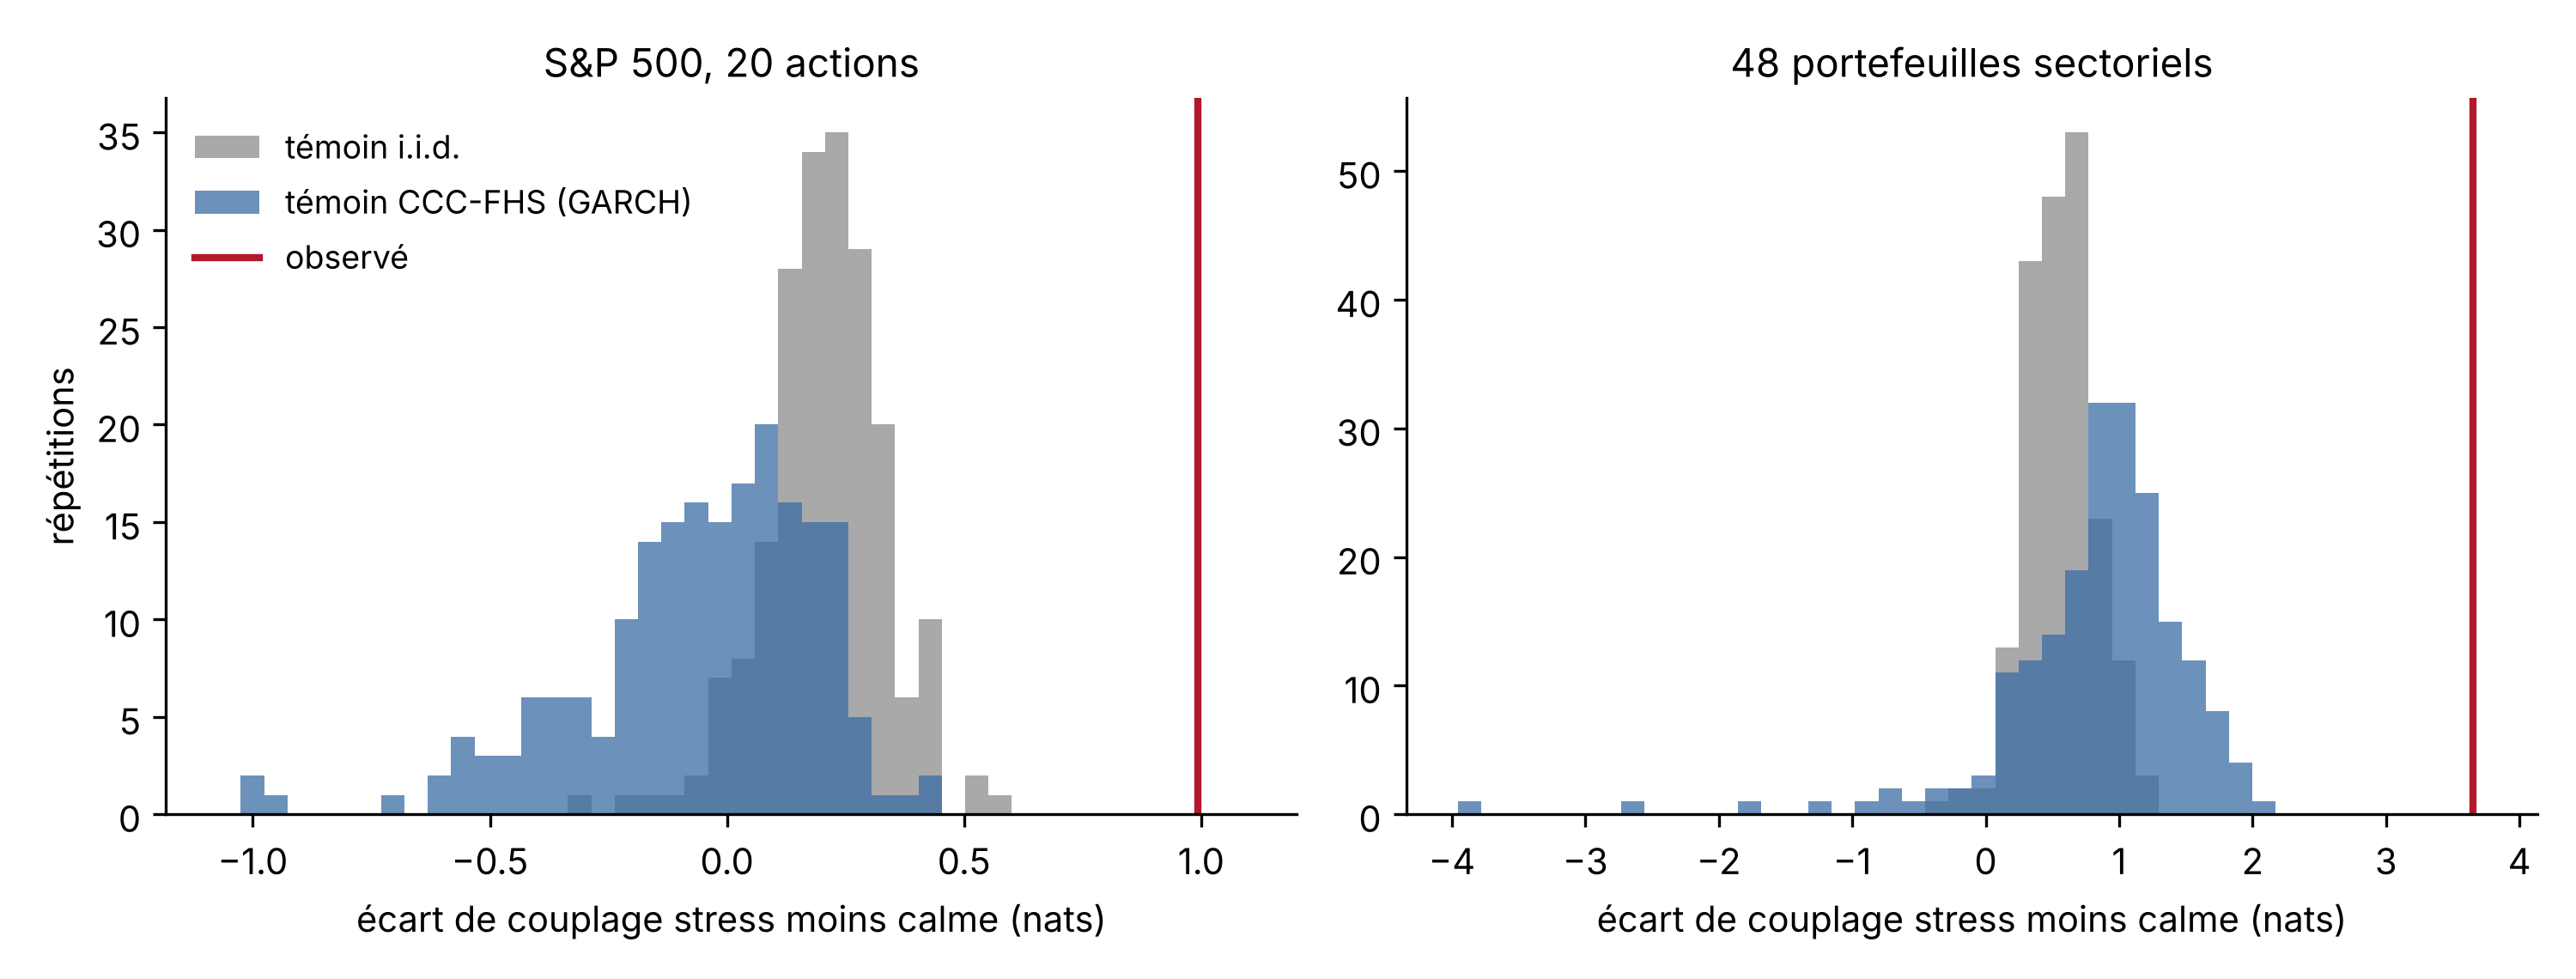
\includegraphics[width=\linewidth]{../figures/fig_null_distributions_fr.png}
\caption{Couplage sous stress face à deux témoins placebo. Chaque panneau
montre l'écart stress moins calme du couplage $C$ (nats ; positif quand les
actifs se couplent sous stress) pour les données observées (trait vertical) et
pour 200 répétitions du témoin i.i.d.\ et du témoin CCC-FHS (GJR-GARCH à
corrélation constante). À gauche : vingt actions du S\&P~500, 1990--2022. À
droite : 48 portefeuilles sectoriels, 1990--2026.\\
\emph{Texte alternatif :} deux histogrammes ; dans chacun, les deux
distributions des témoins sont nettement à gauche d'un trait vertical qui
marque l'écart de couplage observé.}
\label{fig:null}
\end{figure}

\begin{figure}[p]
\centering
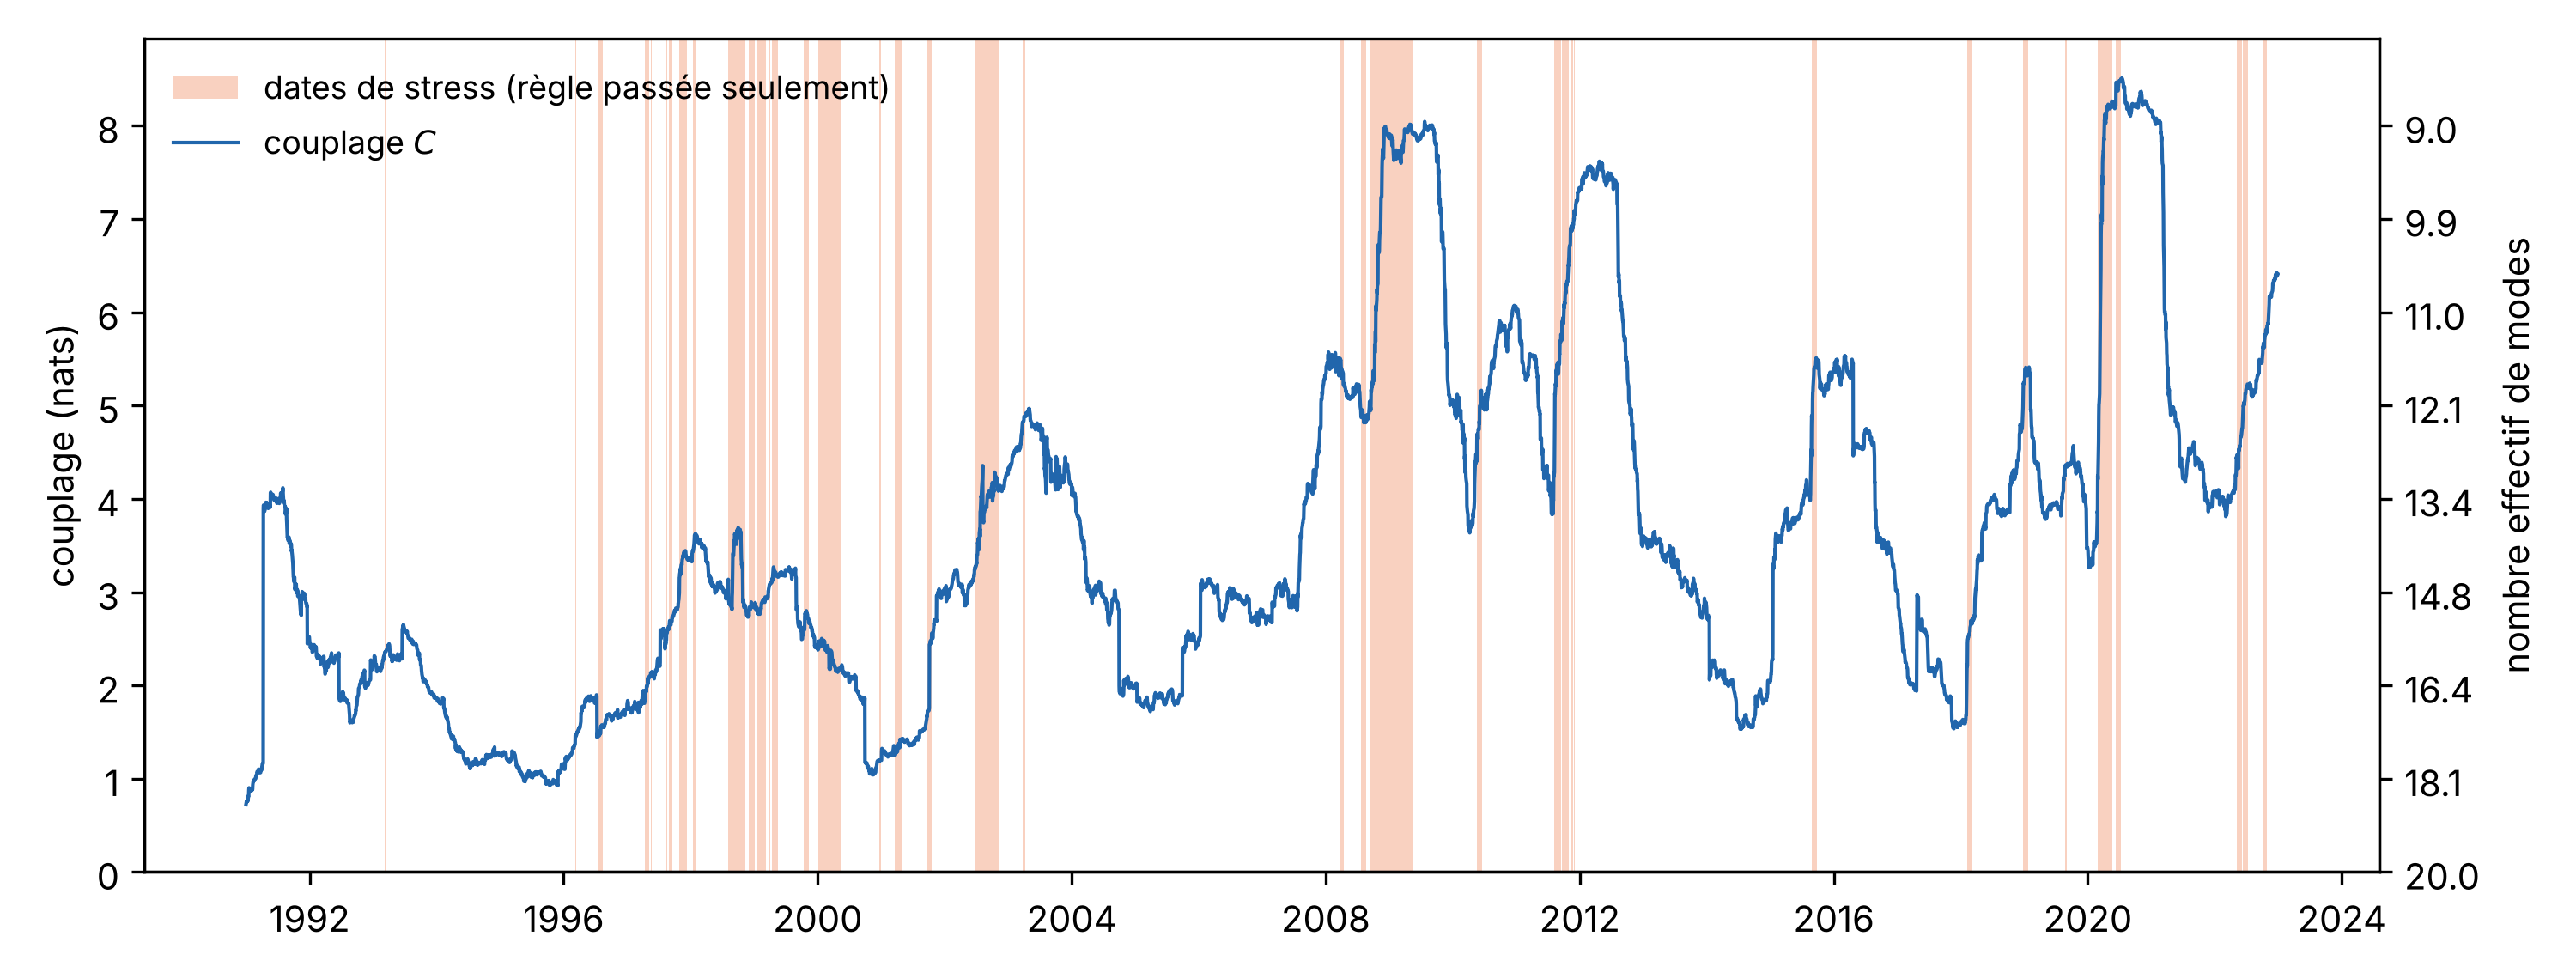
\includegraphics[width=\linewidth]{../figures/fig_coupling_series_fr.png}
\caption{Couplage de vingt actions du S\&P~500, 1990--2022. Couplage glissant
sur 252 jours $C=-\tfrac12\log\det R$ (nats, estimateur de Ledoit--Wolf) et
dates de stress (règle passée seulement) en grisé. L'axe de droite donne le nombre
effectif de modes de risque $N\exp(-2C/N)$.\\
\emph{Texte alternatif :} une série temporelle qui culmine en 2008 et 2020,
alignée sur les périodes de stress grisées.}
\label{fig:series}
\end{figure}

\end{document}
